\section{Application to proplyd bowshocks}
\label{sec:application}

\defcitealias{Canto:1996}{CRW}
\newcommand\CRW{\citetalias{Canto:1996}}

Proplyds are comet-like structures observed in HII regions like Orion Nebula Cluster (ONC). 
These objects are interpreted as a D-type Ionization Front (IF) of a photoevaporated flow 
originated in the protoplanetary disk of a nearby low mass YSO \citep{Johnstone:1998}.
The pressure of the surrounding gas is not enough to confine this flow \citep{HA:1998}
may be formed by the interaction of the photoevaporated wind of the proplyds with the stellar wind of $\theta^1~C~Ori$, which is highly supersonic $(M \sim 100)$. 

The density distribution of the photoevaporated flow can be determined using the steady state continuity equation and assuming that almost all ionizing photons are absorbed at the IF \citep{HA:1998} and ignoring dust absorption, can be found that

\begin{align}
N(r_{IF},\theta) = N_0 \cos^{0.5}\theta
\label{eq:nprop}
\end{align}

Neverthless, we should not restrict to the 0.5 index in equation (\ref{eq:nprop}). We may generalize this relation as follows:

\begin{align}
n(r_{IF},\theta) = n_0 \cos^{k}\theta
\label{eq:ngen}
\end{align}

Where $k >0$ implies that the wind's density decays towards wings, when $k<0$ the wind's density incresases towards the wings and $k=0$ implies that the wind is isotropic.

\subsection{\CRW{} Scenario}
This scenario can be described with the formalism of
\citet[][hereafter \CRW{}]{Canto:1996}, who proposes an algebraic
solution for the two winds interaction problem in the thin shell
approximation, in terms of a free parameter
$\beta\equiv\frac{\dot{M}_wv_w}{\dot{M}_{w1}v_{w1}}$, the winds
momentum ratio, which the quantities with subindex 1 corresponds to
the strongest wind, therefore $\beta<=1$.

If we apply the \CRW{} formalism for a more generalized photoevaporated flow with density given by (\ref{eq:ngen}), we find that the solutions for equations (8) - (11) of \CRW{} are the following:

\begin{align}
\dot{M}_w &= \frac{\dot{M}_w^0}{2(k+1)}\left(1-\cos^{k+1}\theta\right) \label{eq:dotprop} \\
\mathrm{where} & M^0_w \equiv 4\pi v_w r^2_{IF} n_0 \bar{m}\\
\dot{\Pi}_z &= \frac{v_w\dot{M}_w^0}{2(k+2)}\left(1-\cos^{5/2}\theta\right)  \label{eq:pir}\\
\dot{\Pi}_r &= \frac{1}{2}\dot{M}^0_w V_w I_k (\theta) \label{eq:piz}\\
I_k(\theta) & = \int^\theta_0 \cos^k \theta \sin^2\theta~d\theta \\
\dot{J}_w = 0 \label{eq:jdot}
\end{align}  
Combining equations  (\ref{eq:dotprop}) to (\ref{eq:jdot}) with equation (6) of \CRW{}  we can obtain the bow shock shape $R(\theta)$. Actually, we work with two different scenarios:
% as illustred in figure (\ref{fig:r-beta}), where we show the resulting bow shock shapes for two scenarios:
$k=1/2$ ak.a. the ``proplyd case'', following \citep{HA:1998}, and $k=0$, ak.a, the ``isotropic case'', following \CRW{}. The comparison betwwen both solutions is shown in figure (\ref{fig:r-beta}).


% Combining equations (6),(9)-(11) and (19)-(23) from \citep{Canto:1996} and (\ref{eq:nprop}), we can solve numerically for $R(\theta)$, which gives us the shell's shape. Also we can
%obtain a relation between $\theta$ and $\theta_1$

%\begin{align}
%\theta_1\cot\theta_1 = 1+ 2\beta I(\theta)\cot\theta - \frac{4}{5}\beta\left(1-\cos^{5/2}\theta\right)
%\label{eq:th1th}
%\end{align}

%Where $I(\theta)\equiv \int^\theta_0 \cos^{1/2}\theta\sin^2\theta~d\theta$. The solution of this integral is an incomplete elliptical integral of the second kind:

%\begin{align}
%\int^\theta_0 \cos^{1/2}\theta\sin^2\theta~d\theta = \frac{4}{5}E\left(\frac{\theta}{2}|2\right) - \frac{1}{5}\sin 2\theta\cos^{1/2}\theta
%\end{align}

\begin{figure}
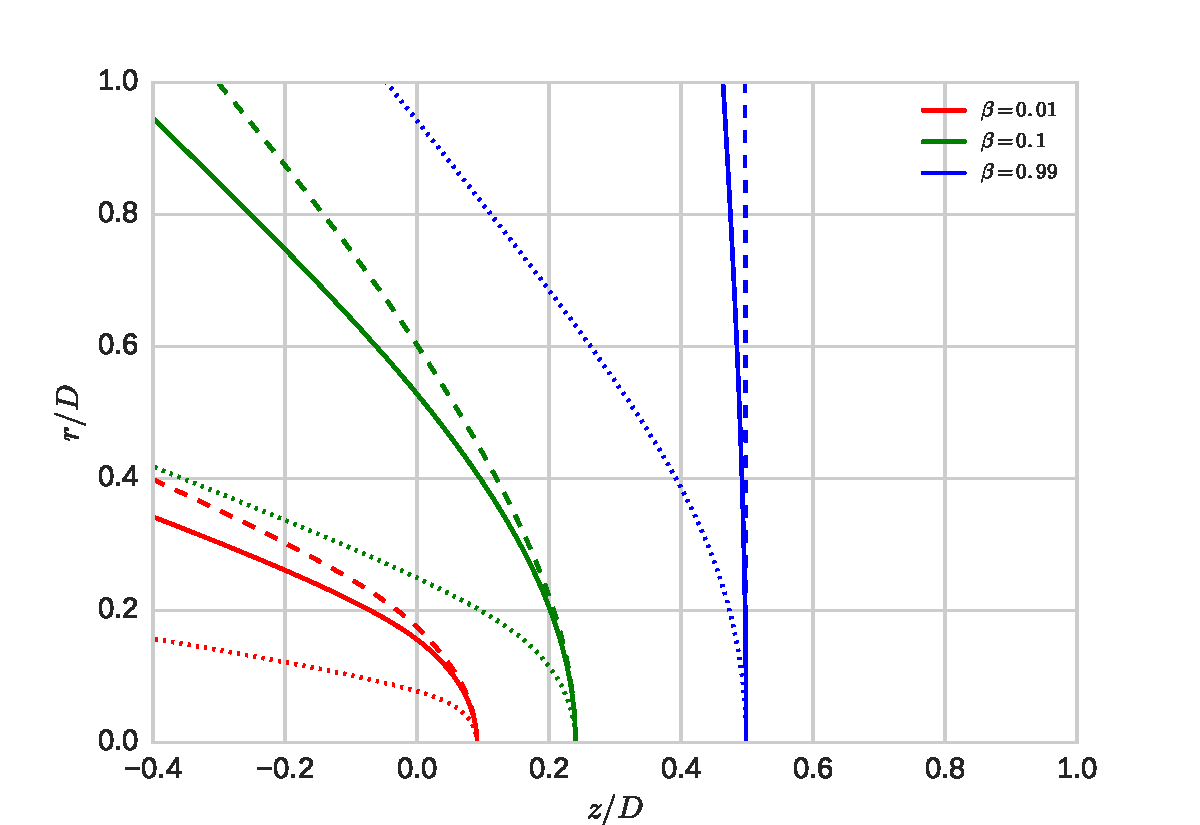
\includegraphics[width=\linewidth]{r-beta}
\caption{Bow shock shapes for interacting winds in the thin-shell
  approximation. Coordinates are normalized by $D$, the distance
  between the two wind sources.  The weaker source is at \((0.0, 0.0)\)
  and the stronger source is at \((1.0, 0.0)\).  Results are shown for
  different values of the wind momentum ratio, \(\beta\), and for the
  case where the weaker wind is isotropic (dashed lines) or an
  anisotropic proplyd photoevaporation flow (solid lines).}
\label{fig:r-beta}
\end{figure}

\subsection{Characteristic Radii}

In order to find an analytic form of the characteristic radii $(R_0,R_c,R_{90})$, we may combine equations (\ref{eq:dotprop}) to (\ref{eq:jdot}) with (6) and (23) from \CRW{}
and obtain the following relation:


\begin{align}
\theta_1\cot\theta_1 -1 = 2\beta I_k(\theta) \cot\theta - \frac{2\beta}{k+2}\left(1-\cos^{k+2}\theta\right)
\label{eq:th1th}
\end{align}

$R_0$ is obtained directly from equation (27) of \CRW{} as the distance from the inner source where the RAM pressure of the interacting winds is in equilibrium.

We can obtain $R_{90}$ by the following process:
Evaluating equations  (\ref{eq:th1th}) and (23) from \CRW{} at $\theta=\frac{\pi}{2}$ we obtain the following:

\begin{align}
R_{90} &= D\tan\theta_{1,90} \\
\theta_{1,90}\cot\theta_{1,90} &= 1-\frac{2\beta}{k+2} \label{eq:th190}
\end{align}
Where $\theta_{1,90}\equiv \theta_1(\frac{\pi}{2})$. Combining both equations and  introducing the parameter 
$\xi\equiv \frac{2}{k+2}$ we have:

\begin{align}
R_{90} &= D\frac{\theta_{1,90}}{1-\xi\beta} 
\end{align}


Solving for $\theta_{1,90}$ from equation (\ref{eq:th190}), using a small angle  approximation, we find that:

\begin{align}
\theta_{1,90} \simeq \left(\frac{3\xi\beta}{1+\frac{1}{5}\xi\beta}\right)^{1/2} \\
\label{eq:th190sol}
\end{align}

With this, we have a solution for $B \equiv \frac{R_{90}}{R_0}$:

\begin{align}
B = \frac{\sqrt(3\xi)\left(1+\beta^{1/2}\right)}{(1-\xi\beta)\left(1+\frac{1}{5}\xi\beta\right)^{1/2}}
\label{eq:B}
\end{align}

Now, to obtaining $R_c$ we expand  (\ref{eq:th1th}) until order 2nd order for small $\theta$ values to find that for such values
$\theta_1 = \beta^{1/2}\theta$

This expansion is valid when k is integer or multiple of 1/2.

Expanding equation (23) from \citep{Canto:1996} and substituting $\theta_1$ we found that:

\begin{align}
R \simeq R_0 \left(1+\frac{1+2\beta^{1/2}}{6}\theta^2\right)
\label{eq:R_approx}
\end{align}

Which lead us to derive the radius of curvature at the symmetry axis:

\begin{equation}
R_c = \frac{3}{2}R_0\left(1-\beta^{1/2}\right)^{-1}
\label{eq:Rcurv}
\end{equation}

--- Rethink if should be included on paper ---
Equations (\ref{eq:r90}),  (\ref{eq:Rcurv}) and (27) from \citep{Canto:1996} are labeled as ``analytic i=0'' in figure (\ref{fig:rad-beta}).

\begin{figure*}
\begin{tabular}{ccc}
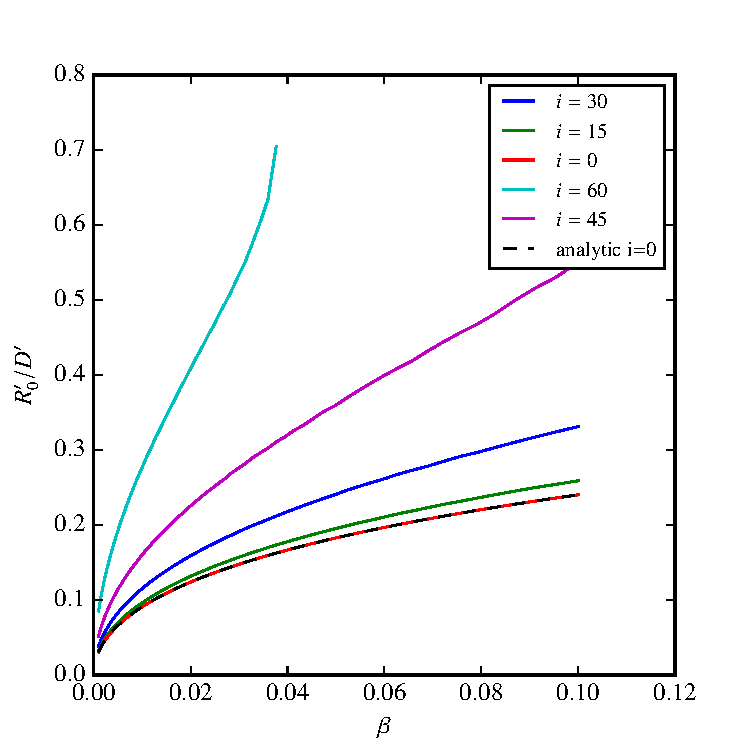
\includegraphics[width=0.35\linewidth]{R0-b}&
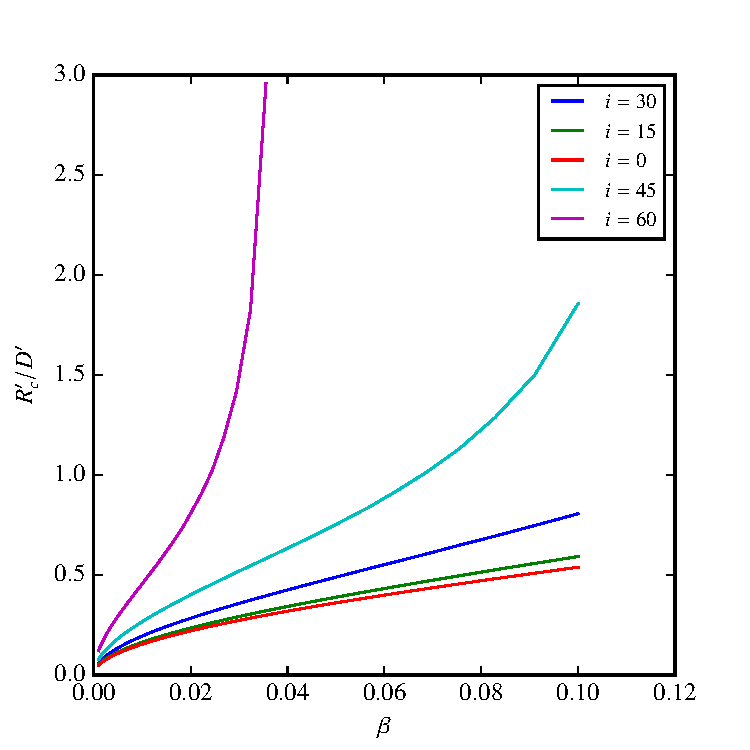
\includegraphics[width=0.35\linewidth]{Rc-b} &
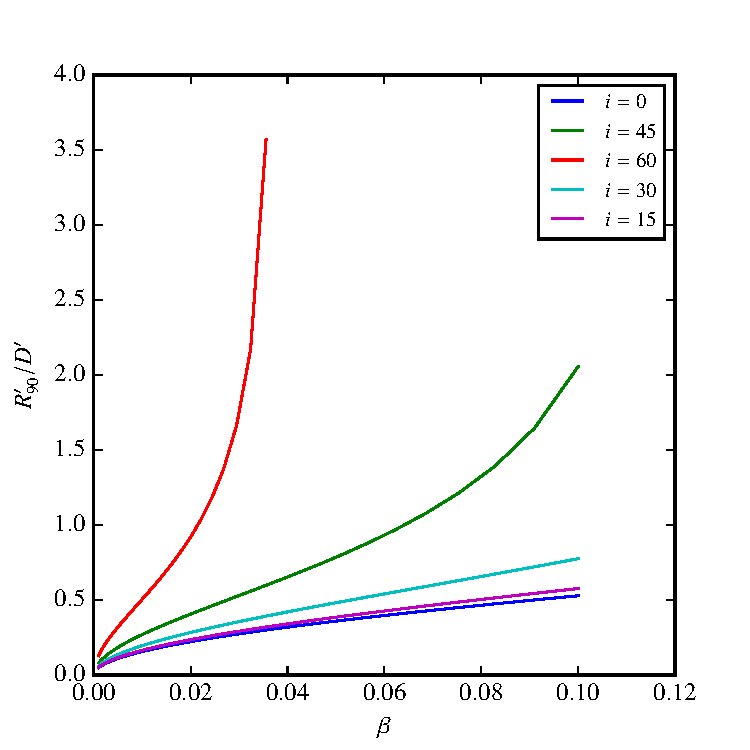
\includegraphics[width=0.35\linewidth]{R90-b}
\end{tabular}
\caption{$R_0$, $R_c$ and $R_{90}$ versus $\beta$ for a fixed set of inclinations. Equations (\ref{eq:r90}), (\ref{eq:Rcurv}), and (27) from \CRW{}
are labeled as ``analytic i=0''. Note that the analytic solution deviates from the numeric solution when $\beta \gtrsim 0.1$}
\label{fig:rad-beta}
\end{figure*}

--- Finished rethinking ---
Observationally, we can measure the projected radii. In order to estimate the model parameters is neccesary to measure at least two of the mentioned radii, being $R_0$ the
easiest to measure. Therefore, we may compare both $R_c$ and $R_{90}$ against $R_0$ as shown in figure (\ref{fig:prop-shell-rad}). 

Although there is an analytical form for the radius of curvature, for $i\ne 0$ there is not an intuitive form for  $R'_c$. Plus, in practice, we are working with discret arrays, so, when transforming the shell's coordinates to the primed system, we almost certainly will miss the $\theta'=0$ point, which
should allow us to estimate the radii $(R'_0,R'_c)$, the first with equation (\ref{eq:Rpar}) and the second with the mathematical definition of the radius of curvature using the primed coordinates. Insted, we estimate $R'_0$ as the projected radius with the value of $\theta'$ closest to zero, and
$R'_c$ doing a least square fit to the points such as $\theta' \leq 45^\circ$. This restriction allows to obtain the best estimation of the radius of curvature at the nos of the shell. A lower cuttoff may undestimate $R'_c$ while higher cutoffs might be unaccurate, too.


 
\subsection{Observational data}

%We measured the Characteristic radii in Orion Nebula proplyds from observations with the ACS camera from the Hubble Space Telescope (HST) using a lamp filter around $\lambda = 5007 \AA$. The proposal for these observations were done by  Jogee, S. in 2004 with calibration purposes but (he never published anything using explicitly these observations). % We must check if this phrase should be included
%Nevertheless, as we are only interested in measure the geometric shape of bow shocks, these observations are more than enough.

\subsubsection{Methodology}
Using the DS9 SAO image tools, we marked the positions of the proplyds and $\theta^1 ~C$. For the shell's position, the marks were placed in the outer border of each shock. 
The number of marks used in each shell varies with shell's size, and with our confidence with our measurements.
Thus, we used few points in small bow shocks and/our the bow shock's outer shell is not well defined. The distance $D$ is measured as the distance between the position of $\theta^1 ~C~Ori$ 
and each proplyd's position. The radius of curvature $R_c$ is measured as the radius of the 
best circle fit of all the data points taken for each proplyd's shell. Finally, we measure $R_0$ as the distance between the proplyd's position and the circle's border in the line which 
include the center of curvature.
To estimate the uncertainties of our measurements, we remove a fraction of the shell's marks, and made 10 sets of randomly chosen removed marks, and made the measurements again to 
see how much these ``variations'' deviates from the original data. The results are summarized and explained in figure (\ref{fig:prop-shell-rad}).  In this figure, in the left side, for each source, 
the fit is done using all the ds9 marks, while in the middle and the right we show two variations removing 2/3 of the marks, but always keeping at least four points. 
In the better observed shells such as 177-341 (top row), the circle
fits are relatively robust to removing points, resulting in little variation between the subsamples. But also there are cases where the variations are more noticeable.



\begin{figure*}
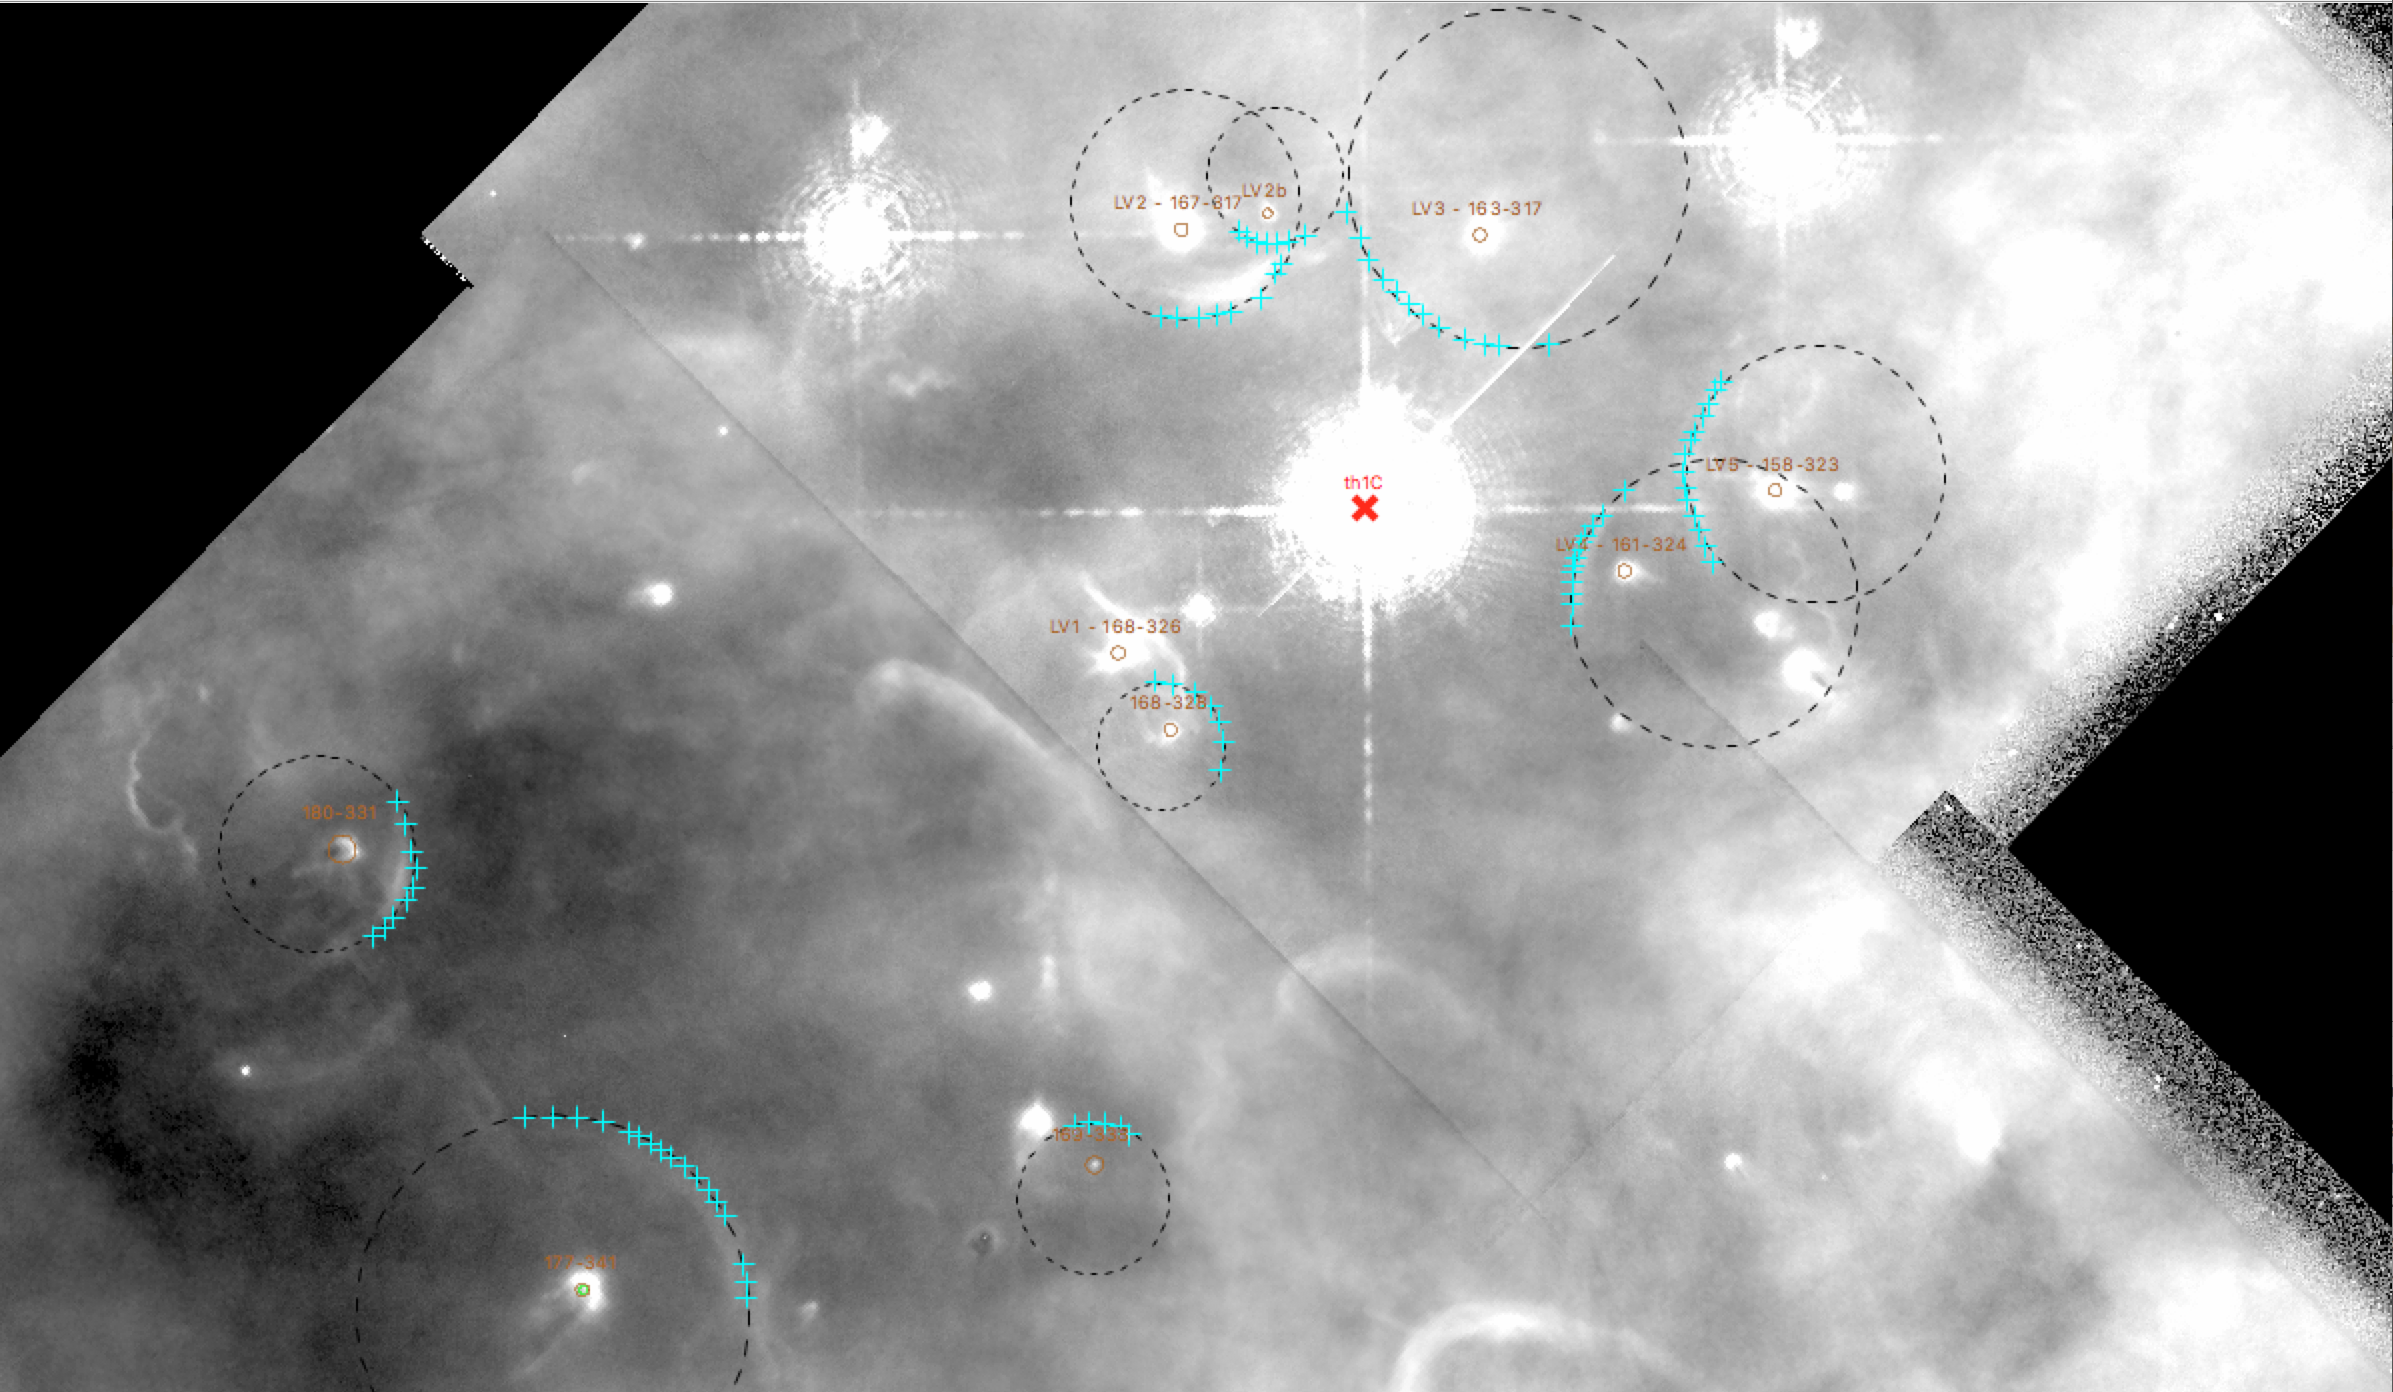
\includegraphics[width=\linewidth]{LV-full-field-annotated.png}
\caption{DS9 shell marks over ONC. The circles mark each proplys position, while the cyan crosses delineate each bow shock and the red X marks the position of $\theta^1 ~C~Ori$. 
The black circles only schematize a circle fit to each shell but they actually are not the real measurements.}
\label{fig:radii-measures-example}
\end{figure*}


\begin{figure}
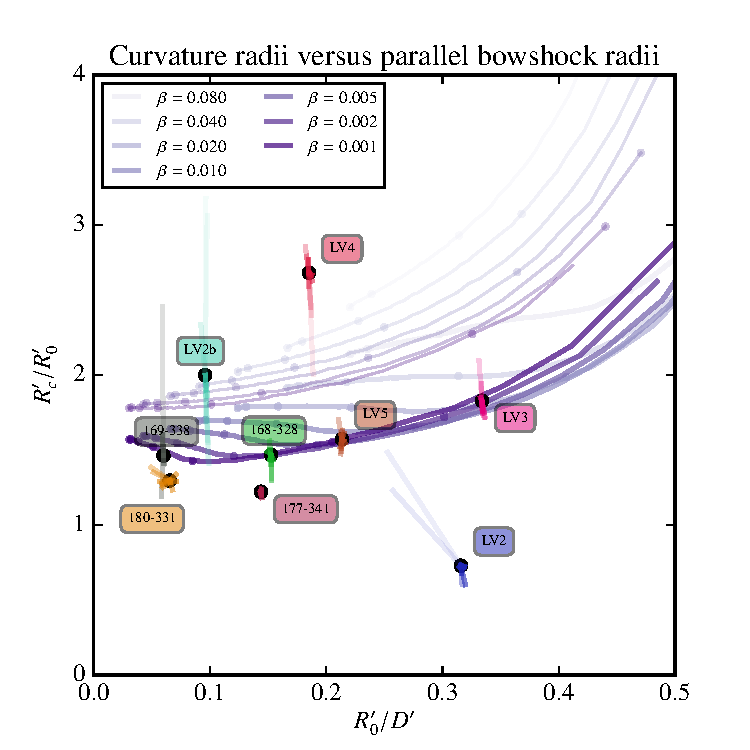
\includegraphics[width=\linewidth]{../../read-shapes/proplyd-shell-R0-Rc-cloud} 
\label{fig:prop-shell-rad}
\caption{Measurements of proplyd's characteristic radii $R_c$ and $R_0$. The curves represent a single bow shock with  fixed wind's momentum ratio $\beta$. 
The dots represent separations in inclination of $15^{\circ}$. The semitransparent curves represent bow shocks which the inner wind is isotropic and the full colored 
curves bow shocks which inner wind density decays as $\cos^{1/2}\theta$. The observational measurements are accompained with radial bars which represents the variations 
with a fraction of the shell's marks removed. Proplyds with less data marks or high asymmetry show higher deviations in the measurements.
%Our measures match far better than \citep{Robberto:2005}, but our data tend to lie at high inclinations $i \gtrsim 45^\circ$, when we expected the opposite. Right side: The same
}
\end{figure}


\begin{figure*}
  \setkeys{Gin}{width=0.33\linewidth, trim=10 30 55 62.5}
\begin{tabular}{@{}c@{}c@{}c@{}}
 
All points & First sub-sample & Second sub-sample \\ 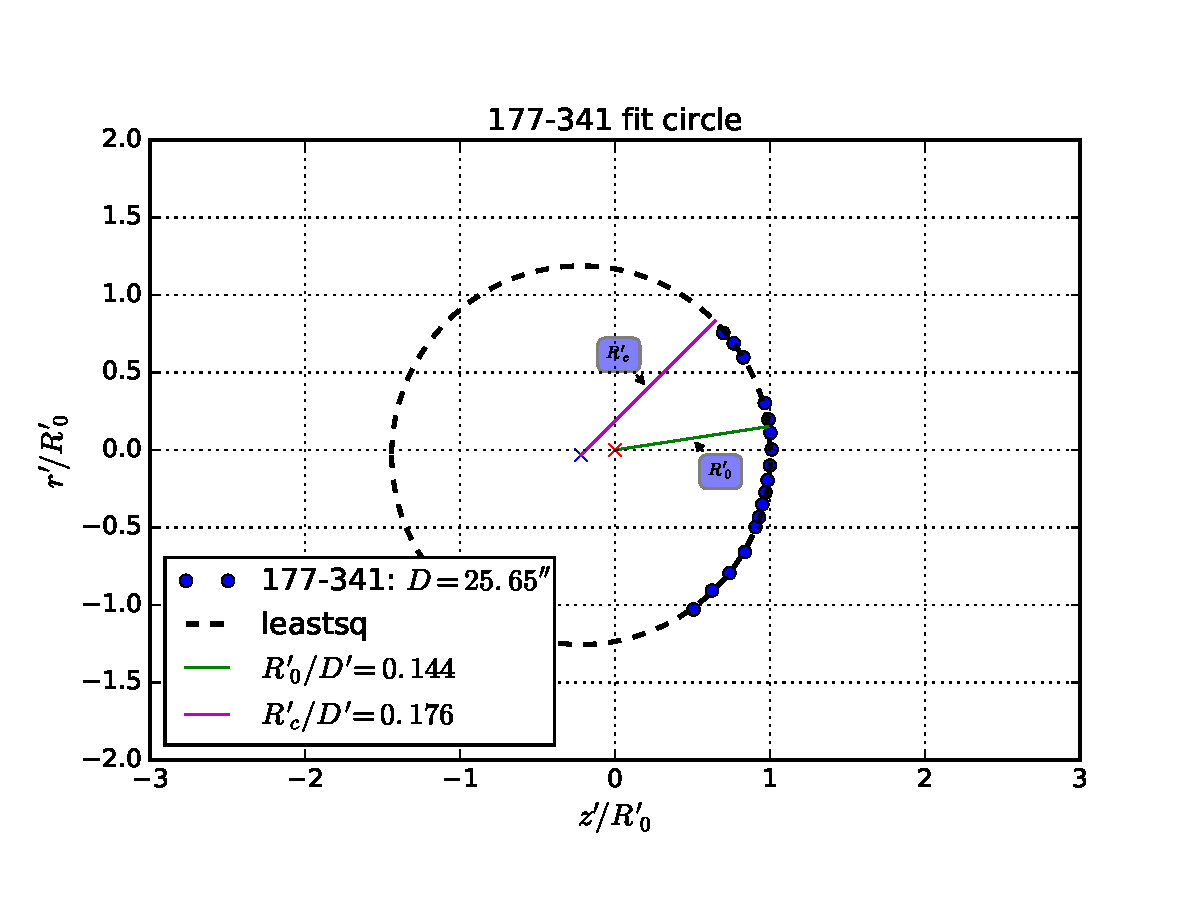
\includegraphics[clip]{../../read-shapes/LV-bowshocks-xyfancy-positionswill-177-341} & 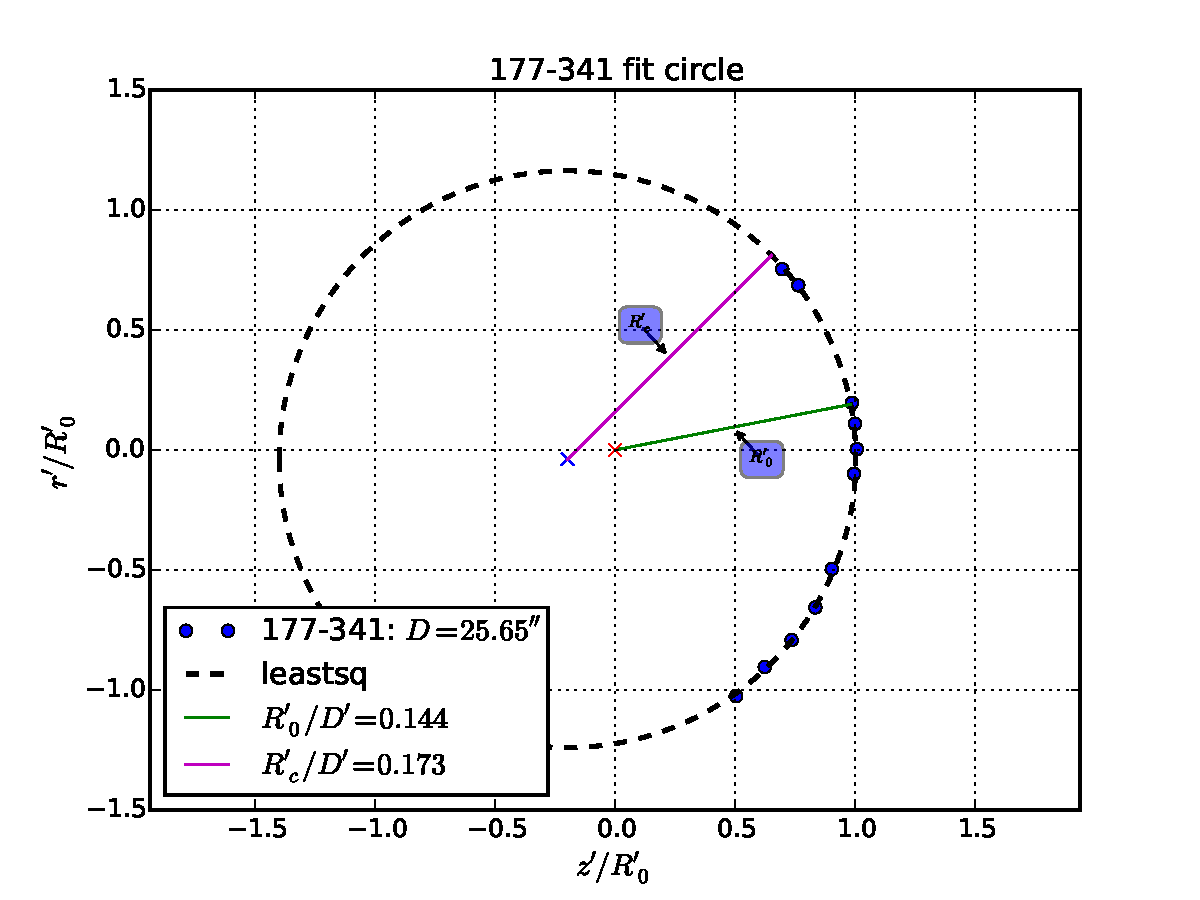
\includegraphics[clip]{../../read-shapes/Multi-Fit/samp00/LV-bowshocks-xyfancy-positionssamp00-177-341} &
  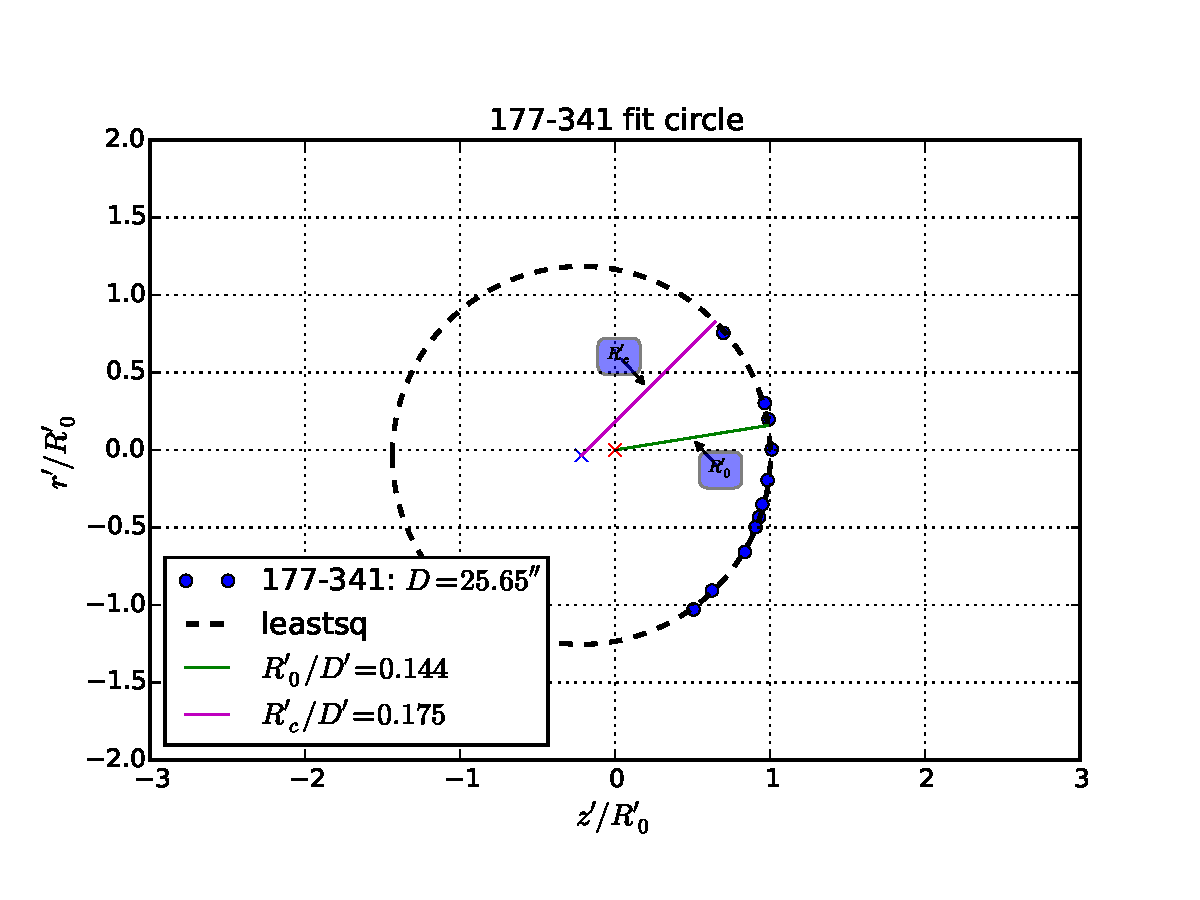
\includegraphics[clip]{../../read-shapes/Multi-Fit/samp01/LV-bowshocks-xyfancy-positionssamp01-177-341} \\
  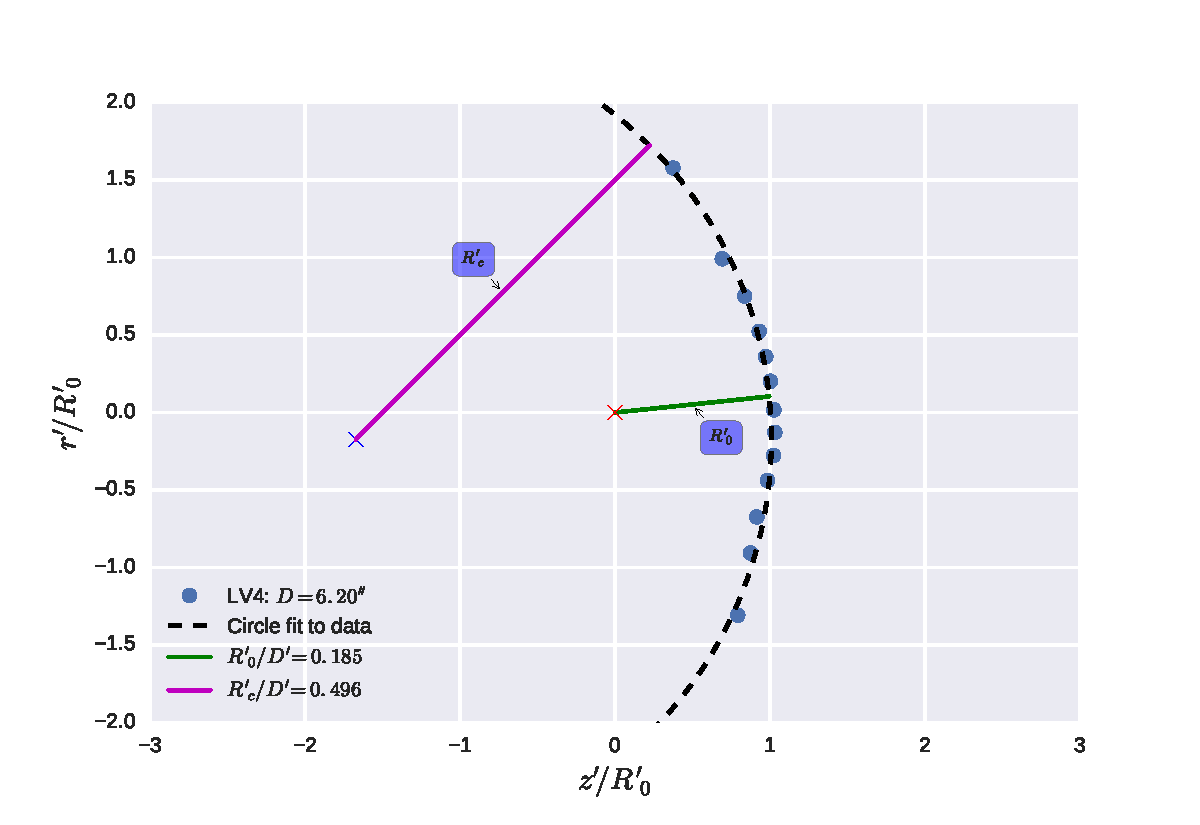
\includegraphics[clip]{../../read-shapes/LV-bowshocks-xyfancy-positionswill-LV4} & 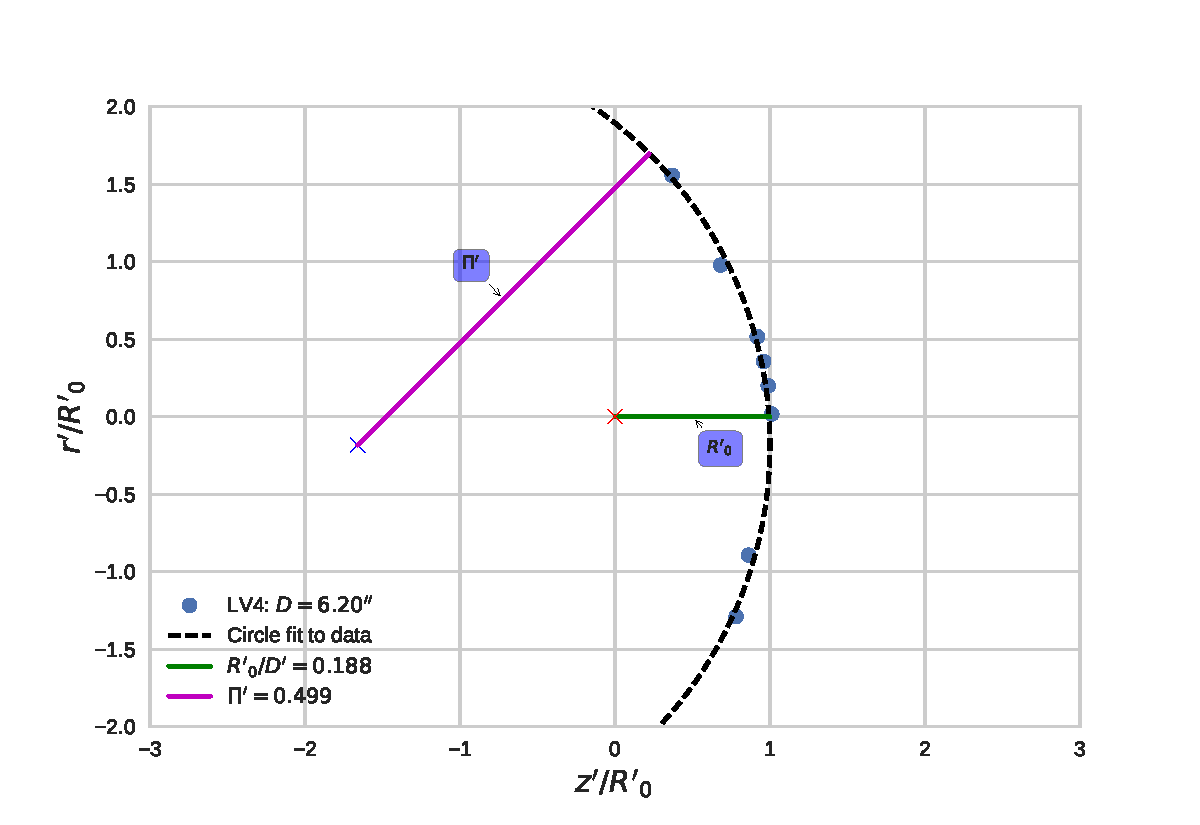
\includegraphics[clip]{../../read-shapes/Multi-Fit/samp05/LV-bowshocks-xyfancy-positionssamp05-LV4} &
  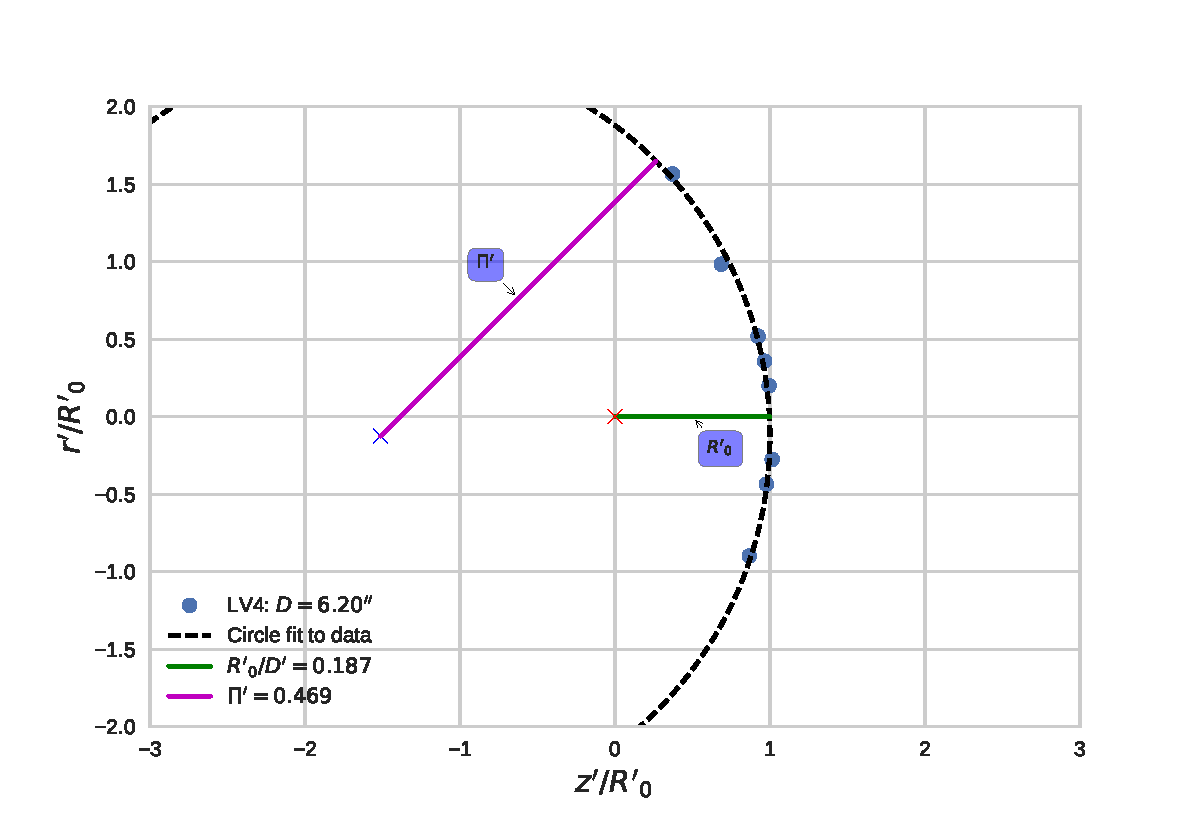
\includegraphics[clip]{../../read-shapes/Multi-Fit/samp01/LV-bowshocks-xyfancy-positionssamp01-LV4} \\
  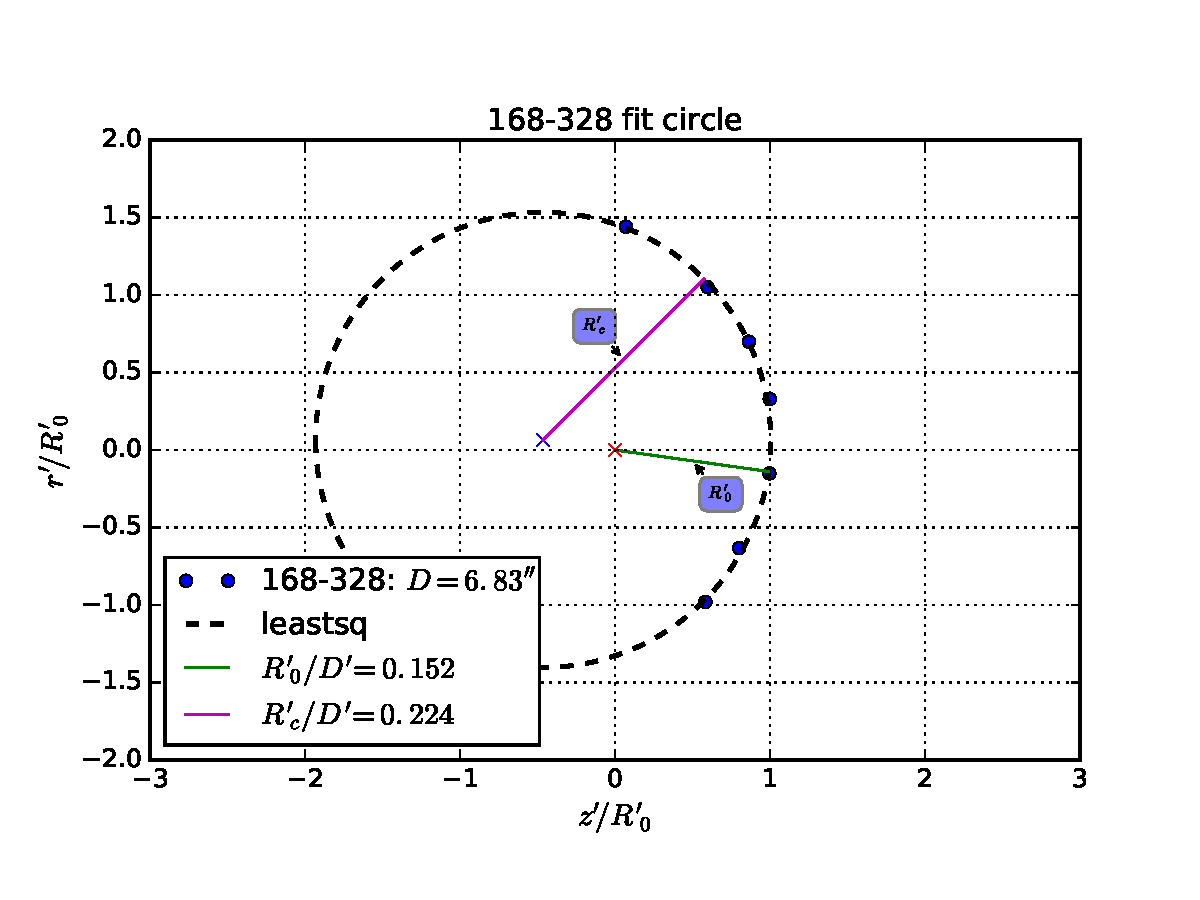
\includegraphics[clip]{../../read-shapes/LV-bowshocks-xyfancy-positionswill-168-328} & 
  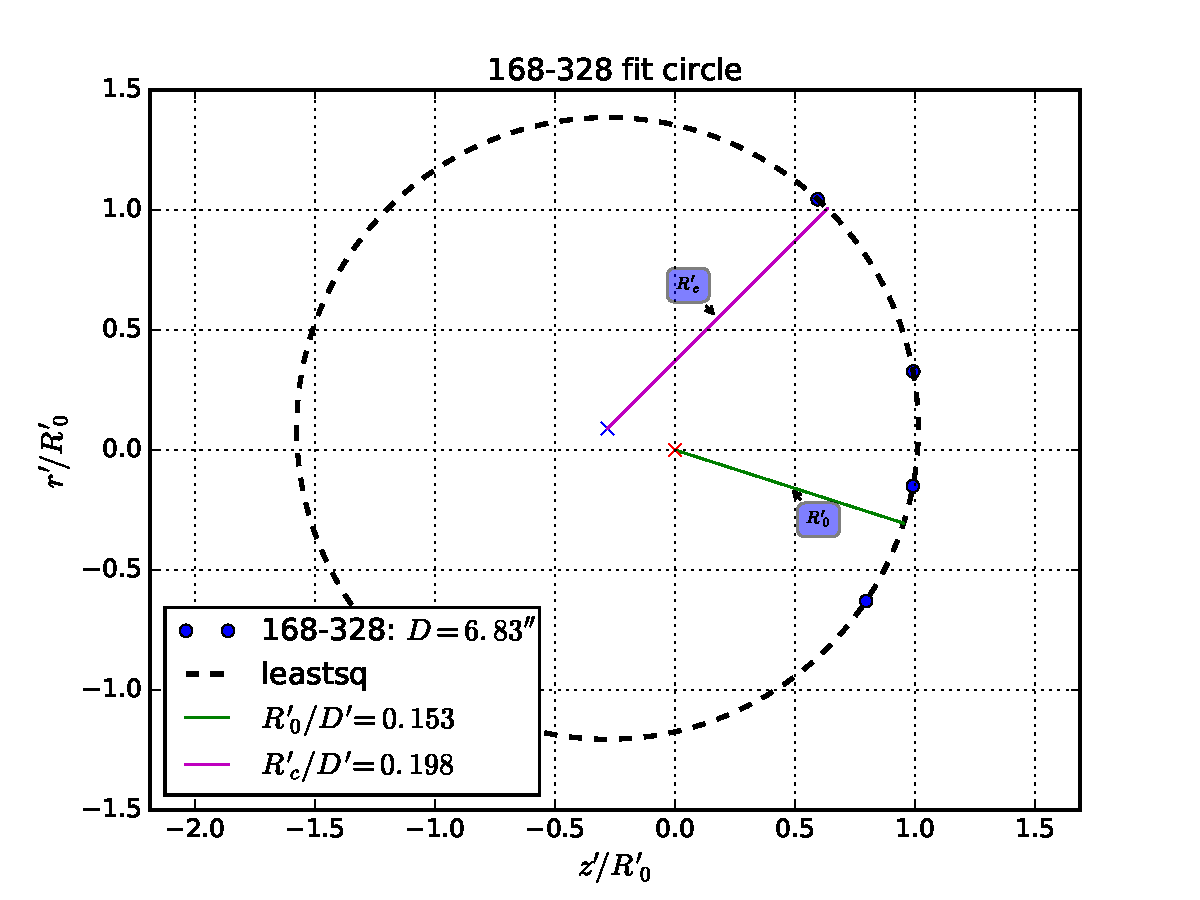
\includegraphics[clip]{../../read-shapes/Multi-Fit/samp00/LV-bowshocks-xyfancy-positionssamp00-168-328} & 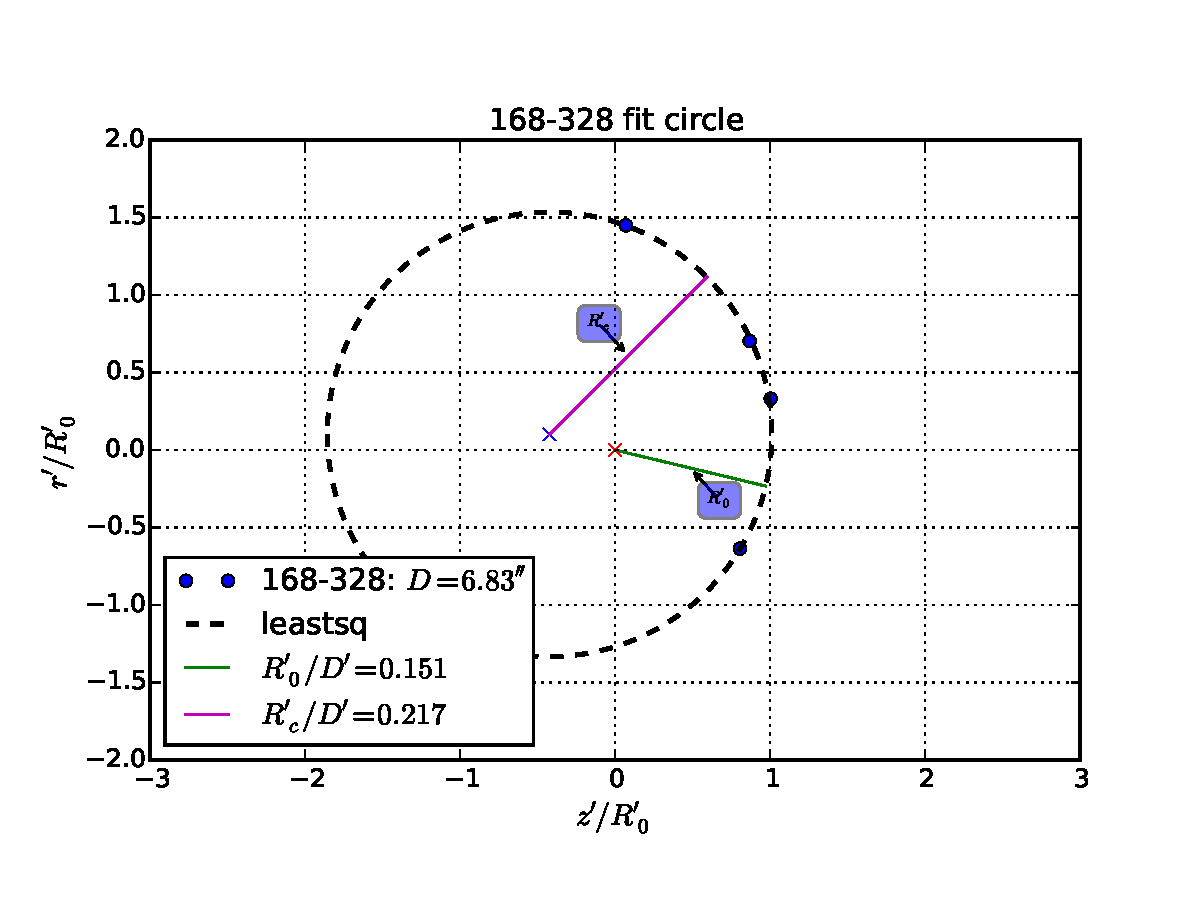
\includegraphics[clip]{../../read-shapes/Multi-Fit/samp01/LV-bowshocks-xyfancy-positionssamp01-168-328}
\end{tabular}
\label{fig:char-radii-obs}
\caption{Examples of systematic uncertainties in the circle fits to
  the shell shapes for three sources (top to bottom rows): 177-341,
  LV4 and 168-328.  The left hand column shows the fit to all of the
  points identified on the shell border, where the number and spacing
  of the points is a subjective measure of our confidence in tracing
  the edge of each shell. The remaining two columns show fits to
  randomly selected sub-samples of 2/3 of the points for each shell.}
\end{figure*}

\subsection{Conic Scenario}

Using equations (\ref{eq:Rcurv}) and (\ref{eq:B}) we can estimate the parameter of conic curves $\theta_c$ as a function of $(\beta,\xi)$ using equation (make it in conics section)

\begin{align}
\tan^2\theta_c &= 3\left| \frac{\xi\left(1+\beta^{1/2}\right)^2}{\left(1-\xi\beta\right)^2\left(1+\frac{1}{5}\xi\beta\right)}-\frac{1}{\left(1-\beta^{1/2}\right)}\right| 
\end{align}

With this we can use the results of section \ref{sec:conic} to estimate the projected conic shapes for bow shocks with different winds momenta and different density distributions. 
In figure (\ref{fig:conic-xi}) we show the theoretical conic curves for different vales of $\beta$ with a fixed $\xi$. Most of the proplyds fit well with a elliptic-like conic shape.
LV4 is a special case which fits better with an hyperbola

\begin{figure*}
\begin{tabular}{cc}
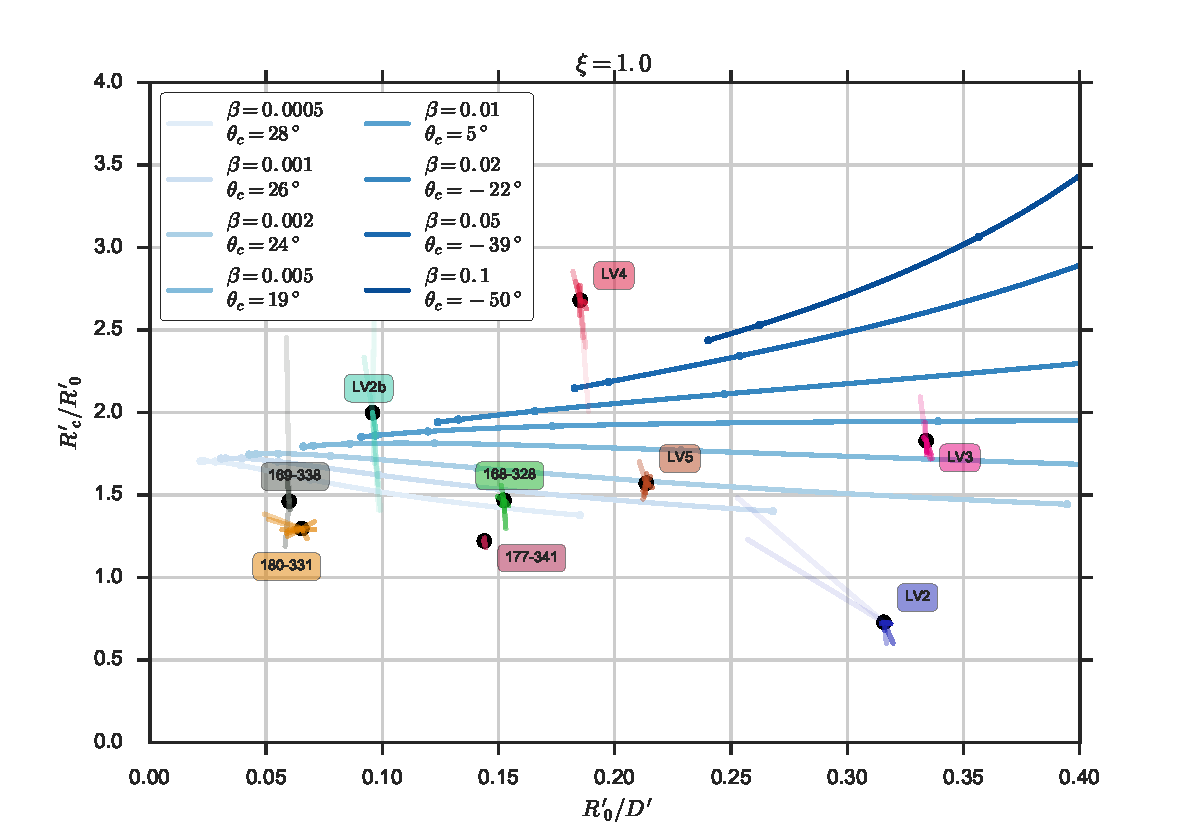
\includegraphics[width=0.48\linewidth]{../../read-shapes/conic_xi-10} & 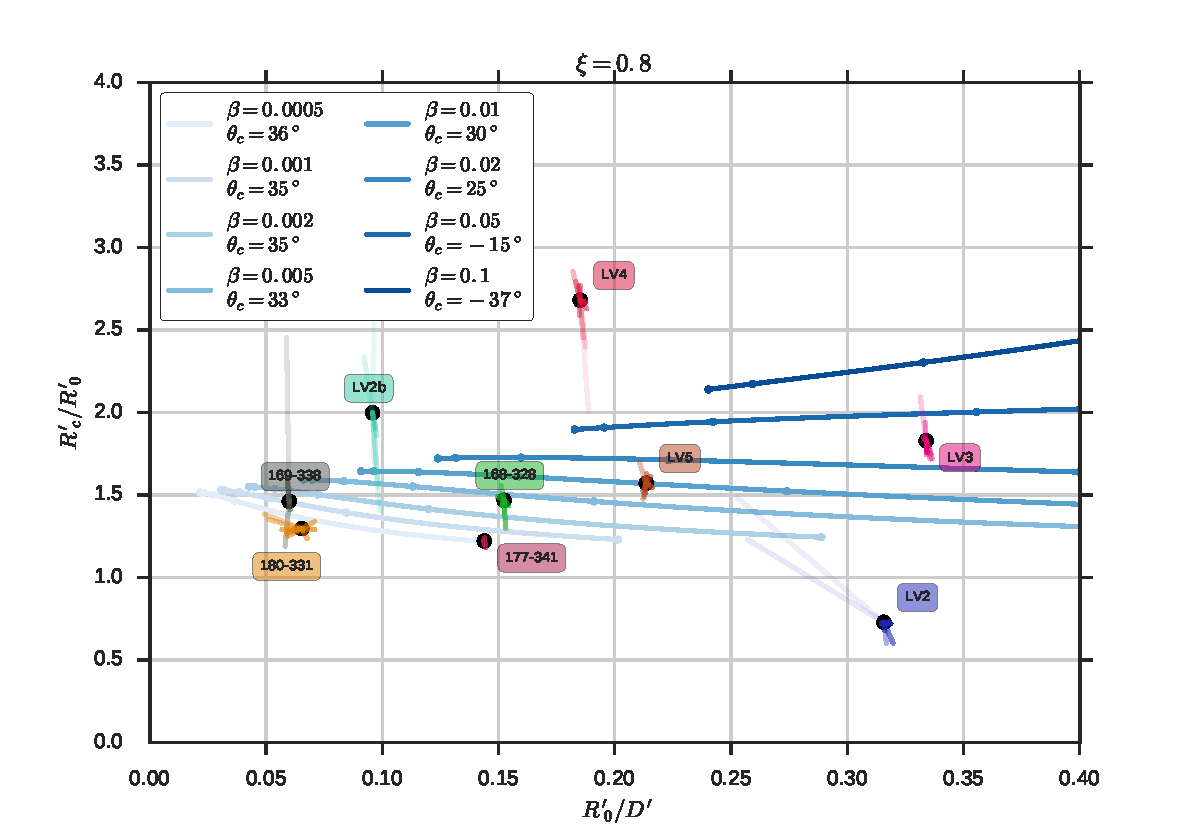
\includegraphics[width=0.48\linewidth]{../../read-shapes/conic_xi-08} \\
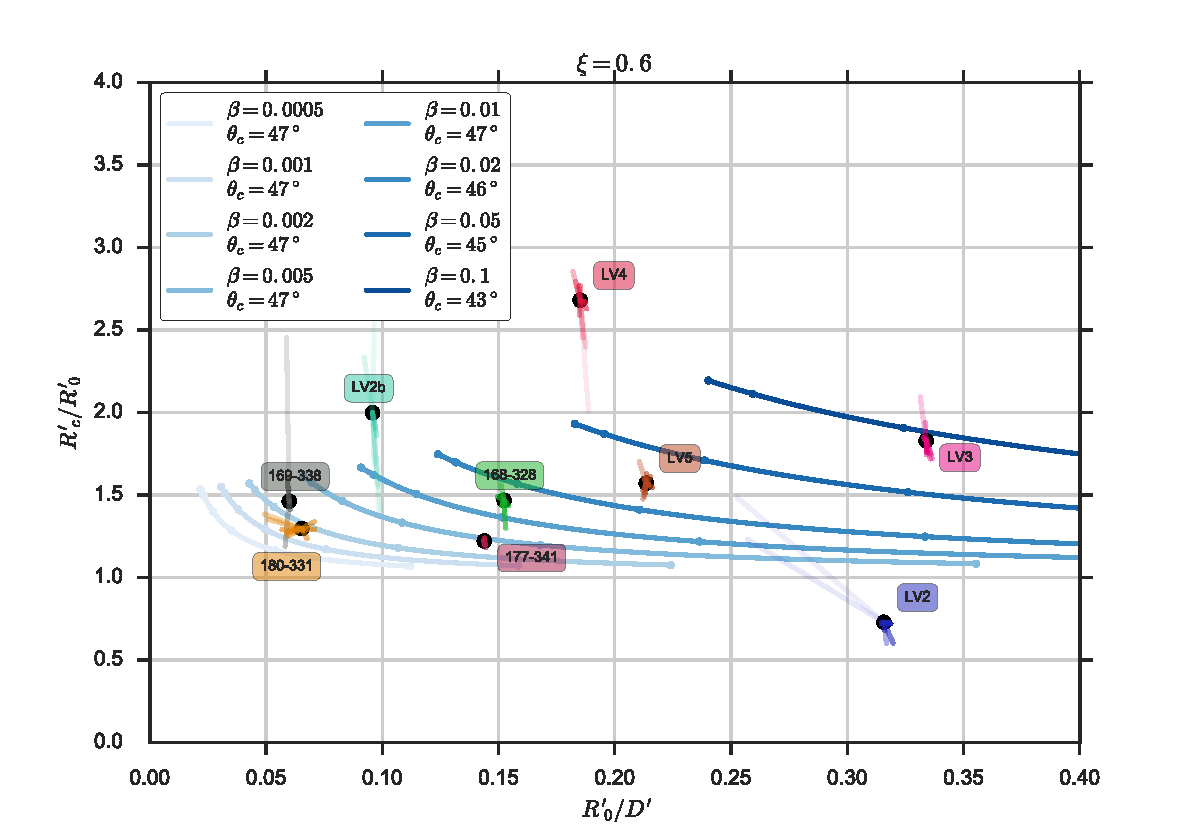
\includegraphics[width=0.48\linewidth]{../../read-shapes/conic_xi-06} & 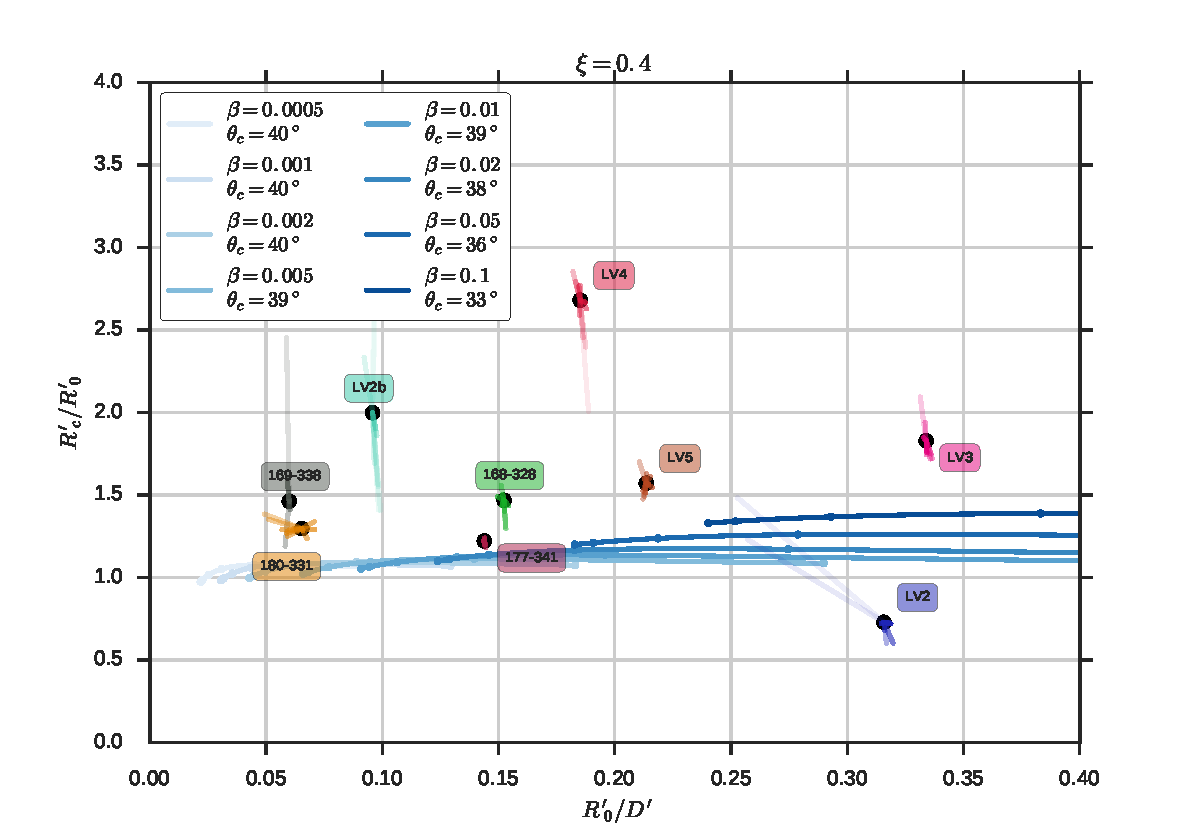
\includegraphics[width=0.48\linewidth]{../../read-shapes/conic_xi-04} 
\end{tabular}
\label{fig:conic-xi}
\caption{Comparison of projected radii for conic models against with the observed proplyds. A fixed value of $\xi$, which describes the anisotropy of the inner wind, is used
in each graph. Models with $\theta_c > 0$ correspond to elliptical-like shapes, while $\theta_c<0$ describes hyperbolic-like shapes.}
\end{figure*}

 \begin{table*}
\begin{tabular}{c|ccccccccc}\hline
Proplyd & LV2 & LV2b & LV3 & LV4  & LV5 & 177-341 & 168-328 & 169-338 & 180-331\\\hline
$D (\arcsec)$ &7.76 & 7.21 &6.89 & 6.2 & 9.55 & 25.65 & 6.83 & 16.43 & 25.07 \\
$R_c/D$  & 0.23  & 0.19& 0.61  & 0.5  & 0.34  & 0.18  & 0.22 & 0.09 & 0.09\\
$R_0/D$  & 0.32 & 0.1 & 0.34 & 0.19 & 0.21 & 0.14 & 0.15 & 0.06 & 0.07\\
$R_c/R_0$ & 0.73 & 2.00 & 1.83 & 2.68  & 1.57 & 1.22 & 1.47 & 1.46 & 1.30  
\end{tabular}
\caption{Characteristic Radii measurements for a sample of proplyds. %Enhance description when more rows were included
} 

\label{tab:proplyds}
\end{table*}

%%% Local Variables:
%%% mode: latex
%%% TeX-master: "proplyd-bowshocks.tex"
%%% End:


%\begin{figure}
%\end{figure} 

%\begin{figure*}
%\begin{tabular}{cc}
%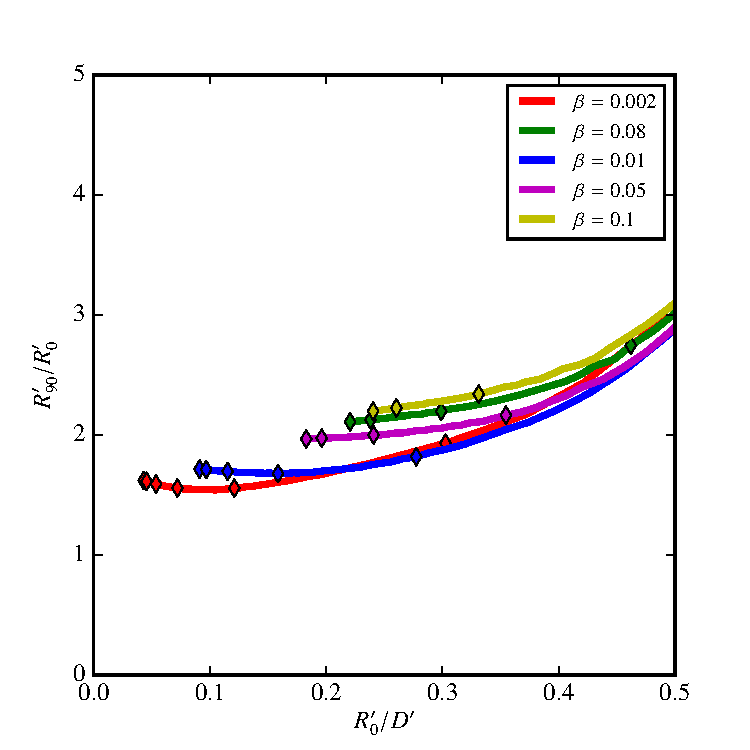
\includegraphics[width=0.5\linewidth]{R90-R0-b}&
%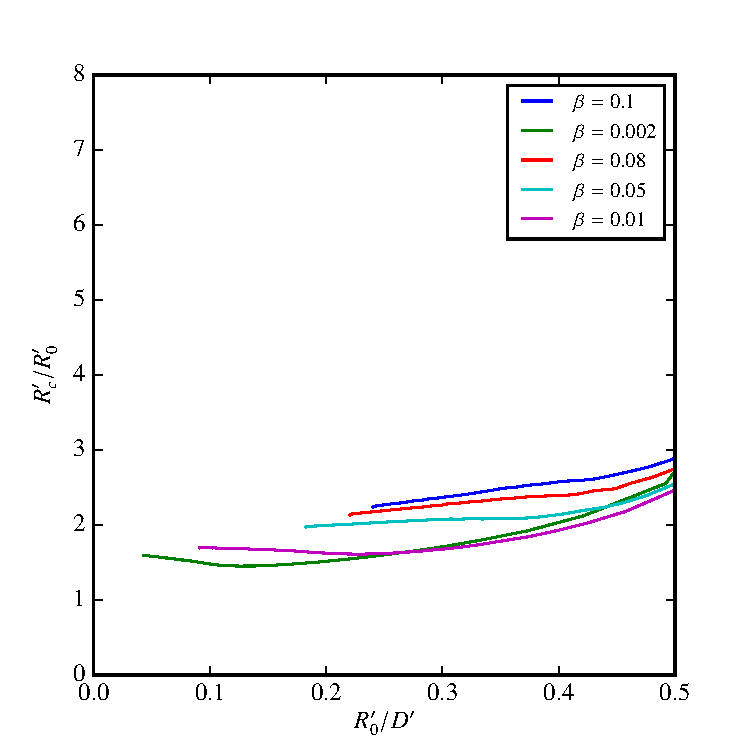
\includegraphics[width=0.5\linewidth]{Rc-R0-b}
%\end{tabular}
%\label{fig:radii-r0}
%\caption{Left: $R_c$ normalized with $R_0$ vs $R_0$ normalized with $D$. Right:$R_{90}$ normalized with $R_0$ vs $R_0$ normalized with $D$. Since the bow shock brightness decays 
%at the wings, it is more difficult to measure $R_{90}$. Along every single curve, $\beta$ is constant. The marks in the curves represents jumps of $15^\circ$ in inclination, and the most left 
%mark in each curve represent $i=0^\circ$}
%\end{figure*}

%is $(0,0)$ and measured distances in arcseconds. In this reference, the proplyd-$\theta_1^C$ line is $y=0$. With the shell's positions, we optimize a circle, whose radius is $R_c$, but
%this optimization has two variants: the first one with the restriction that the center of the circle must lie in the symmetry axis (y=0), and the second variation is with no restrictions. $R_0$ is calculated as the distance between the proplyd position and the bow shock in a line which is also included the
%center of curvature. The figure (\ref{fig:radii-measures-example}) shows a representation of the metodology described. 
%Our first goal was comparing measurements of $(R_0,R_{90})$ of the LV group of proplyds in mid infrared by \citep{Robberto:2005} against observations in [OIII] with better angular resolution but less contrast against
%the background.
%In \citep{Robberto:2005} they compare their observations with shells obtained with the \citep{Canto:1996} two winds interactions formalism. They found no concordance between the model and observations. We attempted to redo the measurements with better resolution observations. We found quickly that we cannot measure $R_{90}$ in a reliable way since the shell's brightness decays toward the wings. Also, we are using a more sophisticated model where the proplyd's wind density decays as $n \propto \cos {1/2}\theta$ instead of an isotropic wind.
%A better replacement of $R_{90}$ is the radius of curvature, defined as the radius of the circle that fits the observations, because always is measurable. Figures (\ref{fig:char-radii-obs}) and (\ref{fig:char-radii-obs-2}) show our measurements of the radius of curvature for the LV group, with exception of LV1, which actually is a binary proplyd, thus our model is not adequate in this case. Also we include the proplyds 167-328, 169-338, 177-341 (HST1), 189-339 and 180-331 which are close enough to $\theta^1~\mathrm{C~Ori}$ to be influenced by it stellar wind.
%Our results show a better concordance (but still not perfect) between models and observations, as shown in figure (\ref{fig:prop-shell-err}). A possible cause of the discrepancy may be that the \citep{Canto:1996} model assumes that the interacting winds are hypersonic in such way that the shocked gas can be considered as a bidimensional surface. In practice, the bow shock has a finite width, which can afect the apparent shape due to projection effects

%Initially we tried to measure the radii $(R_0,R_{90})$, but it wasn't possible due to the fact that the brightness of the shell decays rapidly towards the wings, and using $R_\theta$ where $60 \lesssim \theta < 0 $ is not so useful, because there is not a significant difference between $R_0$ and $R_\theta$. Instead, we introduced the radius of curvature after we realized how well the shell's marks fits into a circle for all the proplyds (see figure (\ref{fig:char-radii-obs})).

%\begin{figure*}
%\begin{tabular}{cc}
%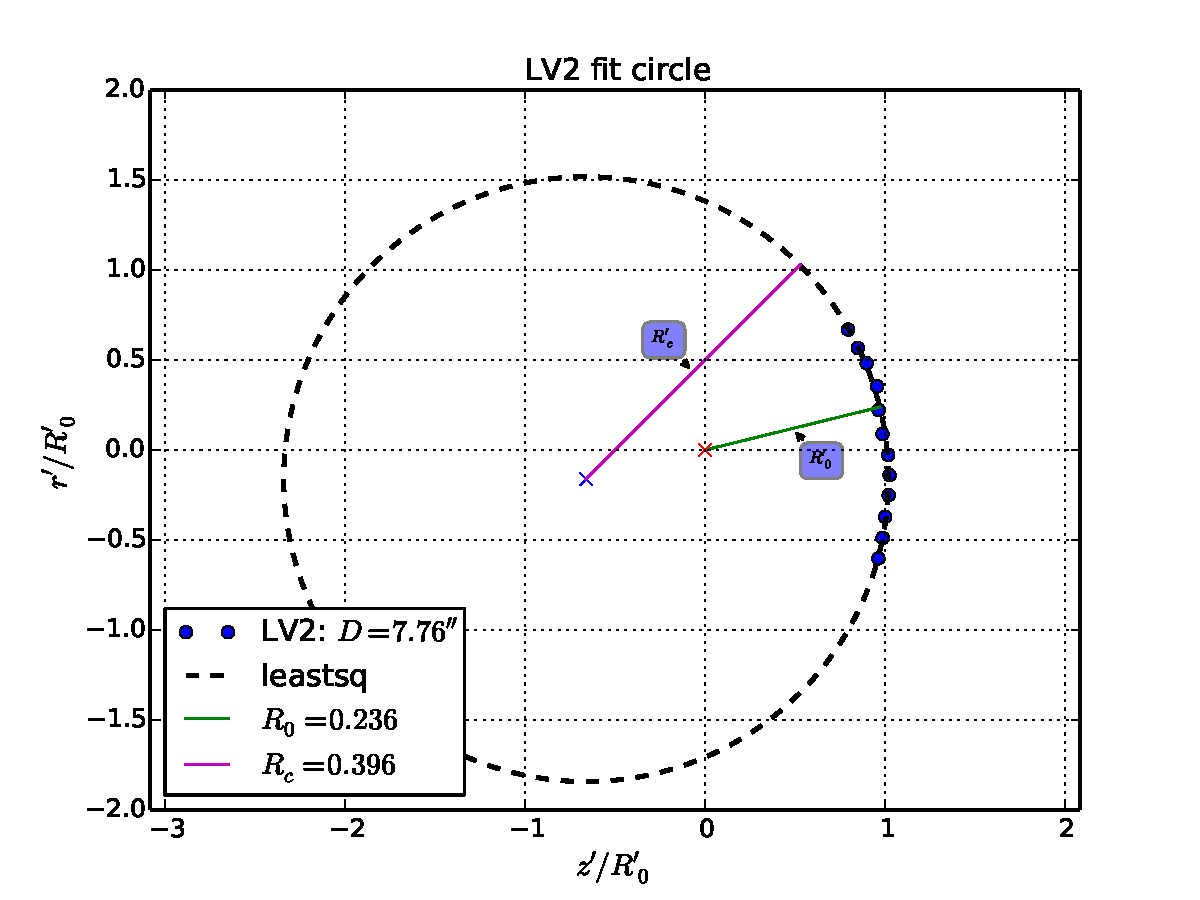
\includegraphics[width=0.5\linewidth]{LV-bowshocks-xyfancy-502epositions-LV2} & 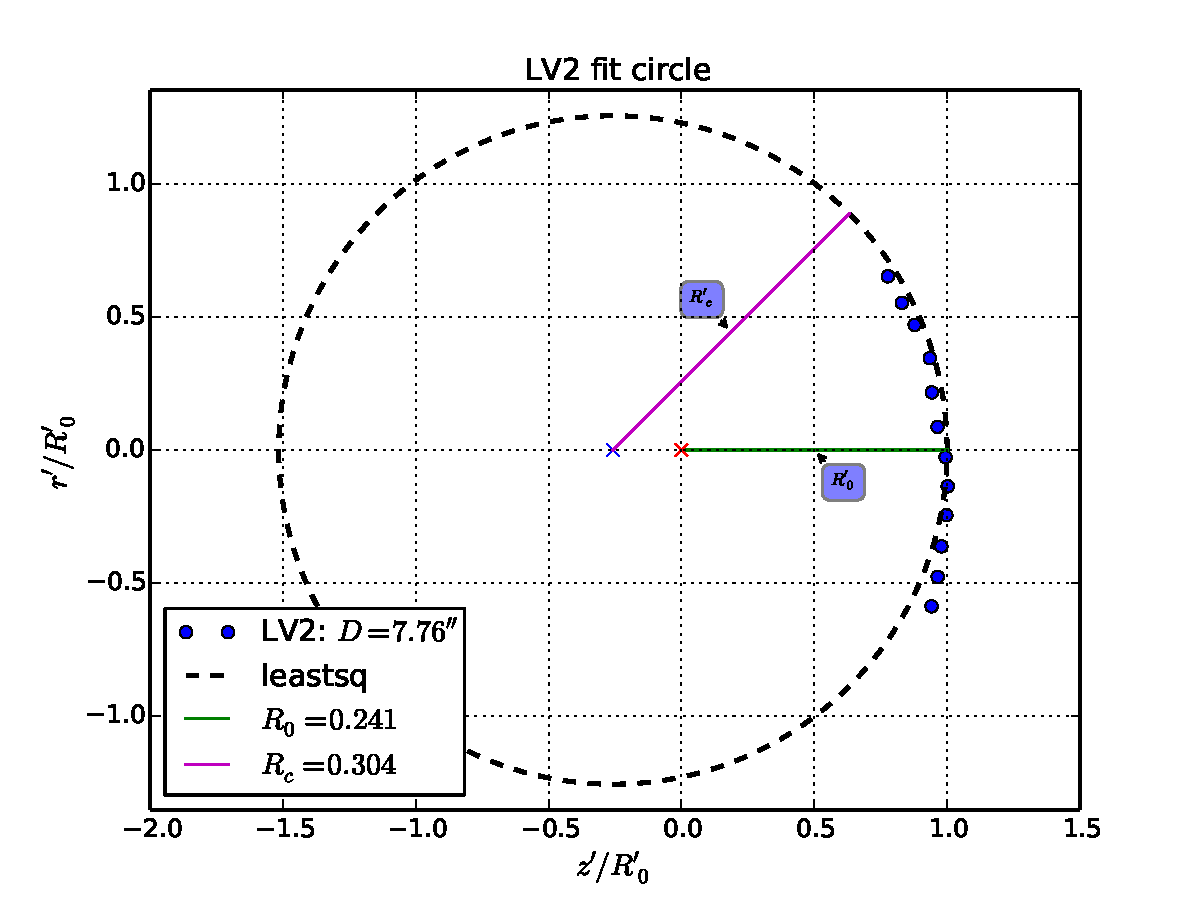
\includegraphics[width=0.5\linewidth]{LV-bowshocks-xyfancy-onaxis-502epositions-LV2} \\
%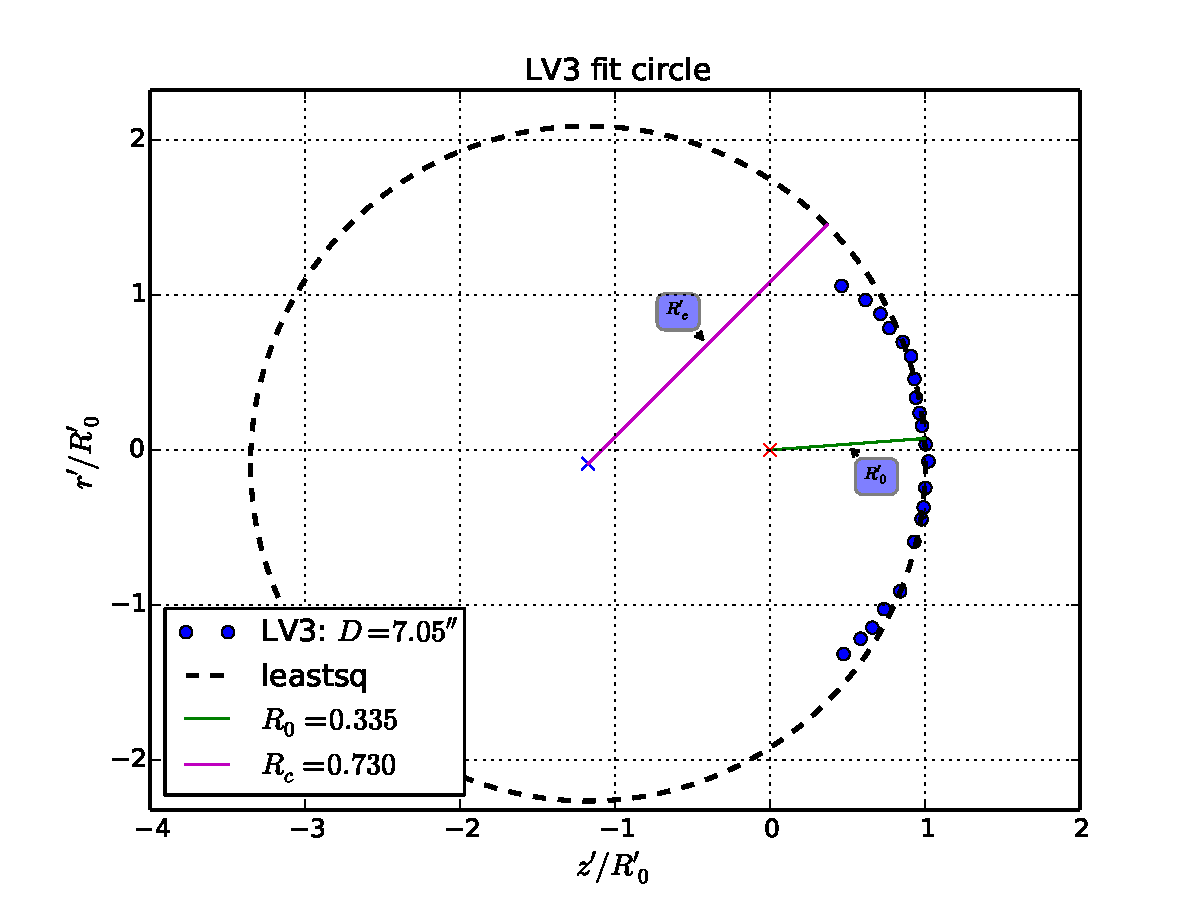
\includegraphics[width=0.5\linewidth]{LV-bowshocks-xyfancy-OIII3a-LV3} & 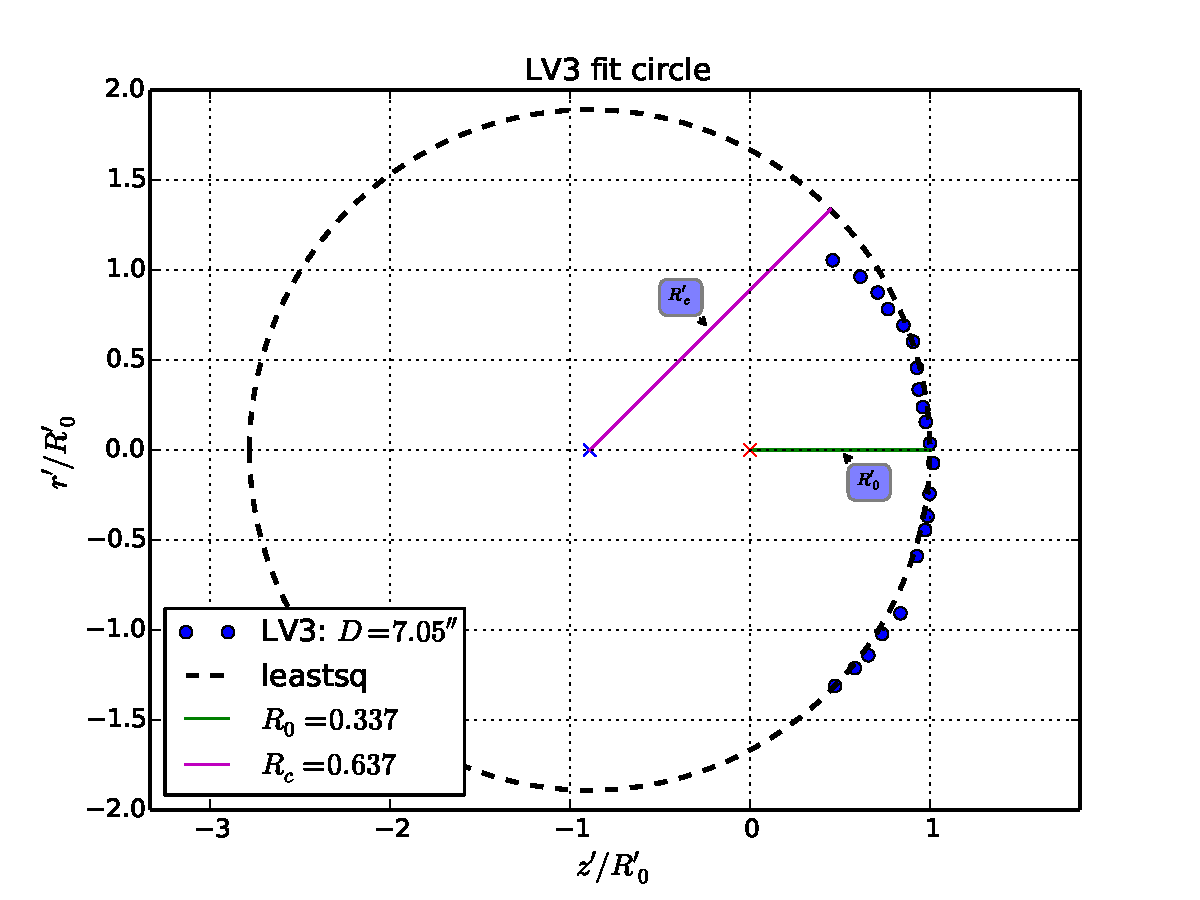
\includegraphics[width=0.5\linewidth]{LV-bowshocks-xyfancy-onaxis-OIII3a-LV3} \\
%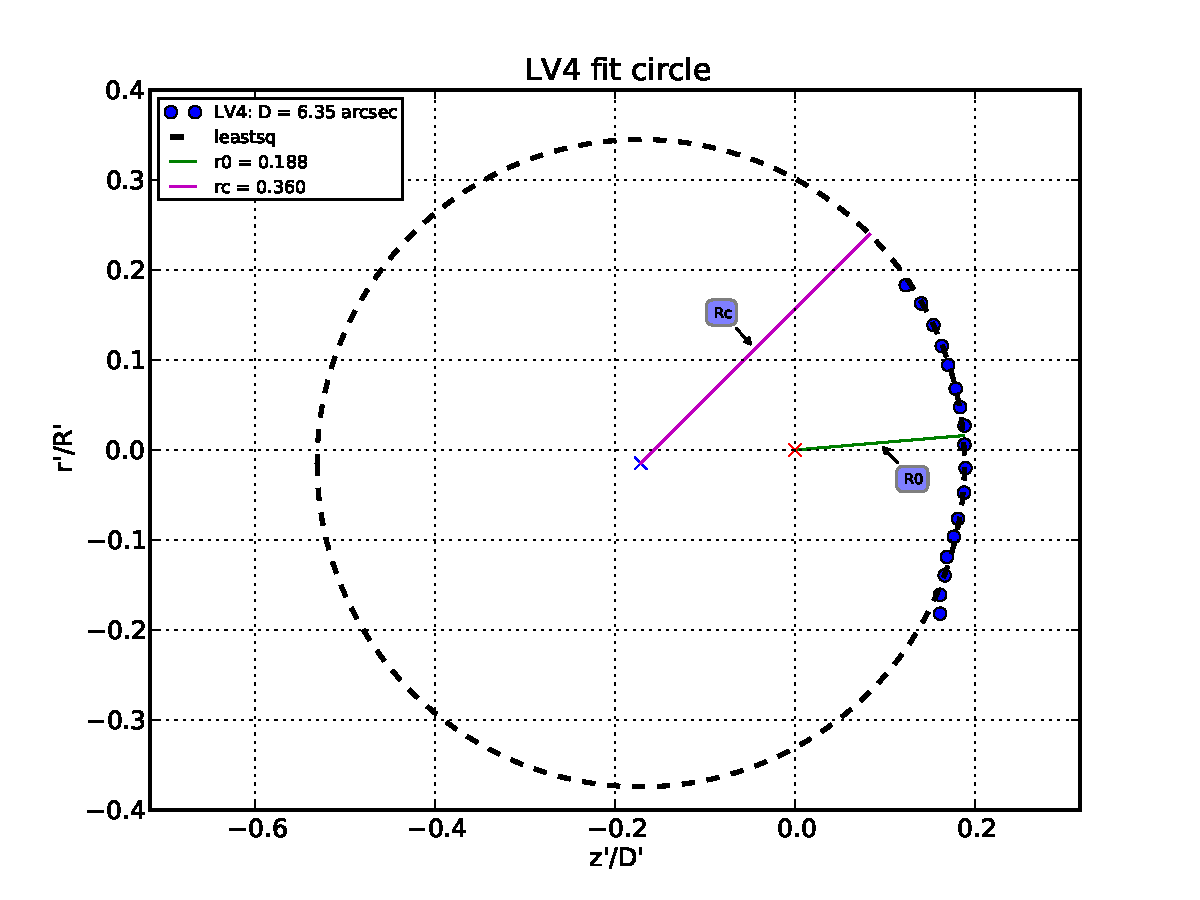
\includegraphics[width=0.5\linewidth]{LV-bowshocks-xyfancy-OIII3a-LV4} & 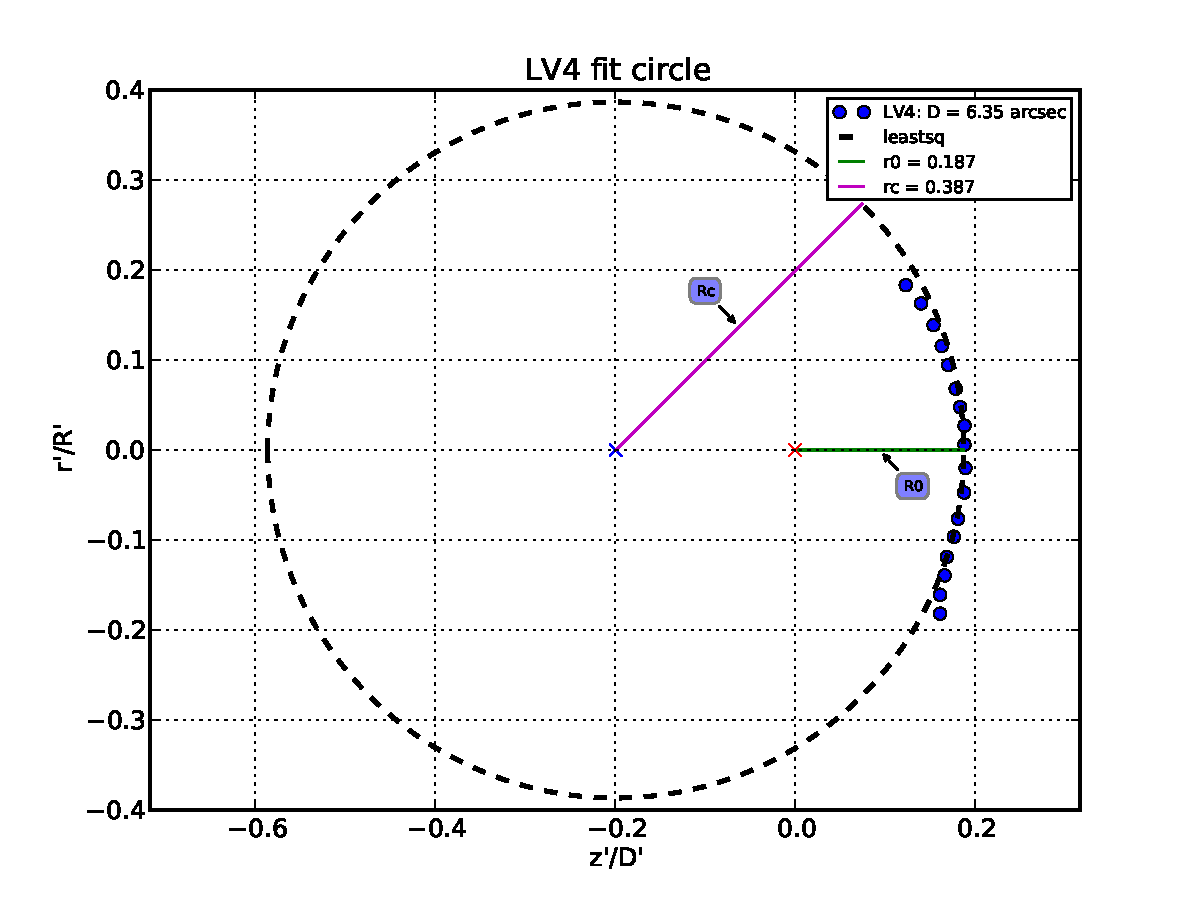
\includegraphics[width=0.5\linewidth]{LV-bowshocks-xyfancy-onaxis-OIII3a-LV4}
%\end{tabular}
%\label{fig:char-radii-obs}
%\caption{Fits to the shell's shapes. In the left side we have the fits without any restrictions. In the right side we have the fits restricting the center of the circle to be in $y=0$. This data is summarized in table (\ref{tab:proplyds})}
%\end{figure*}

%\begin{figure*}
%\begin{tabular}{cc}
%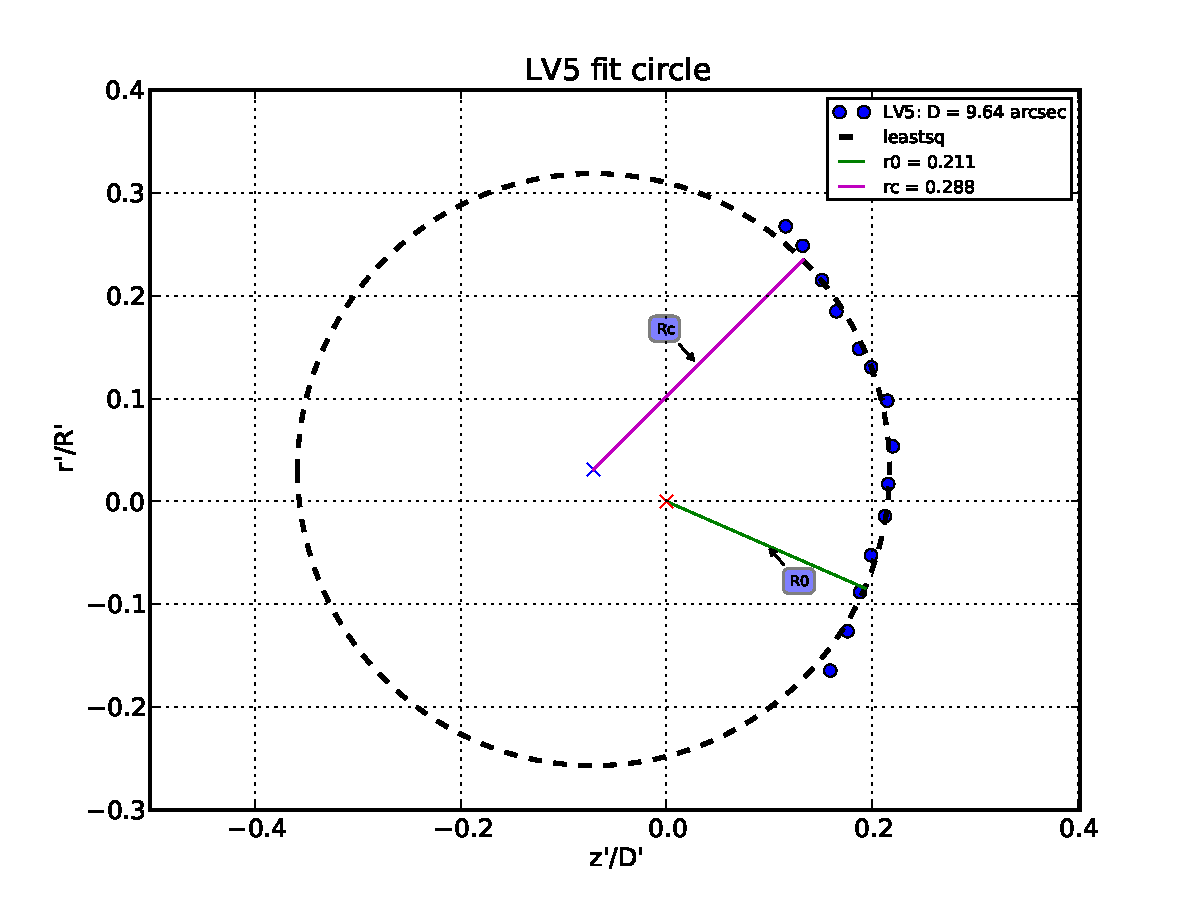
\includegraphics[width=0.5\linewidth]{LV-bowshocks-xyfancy-OIII3a-LV5} & 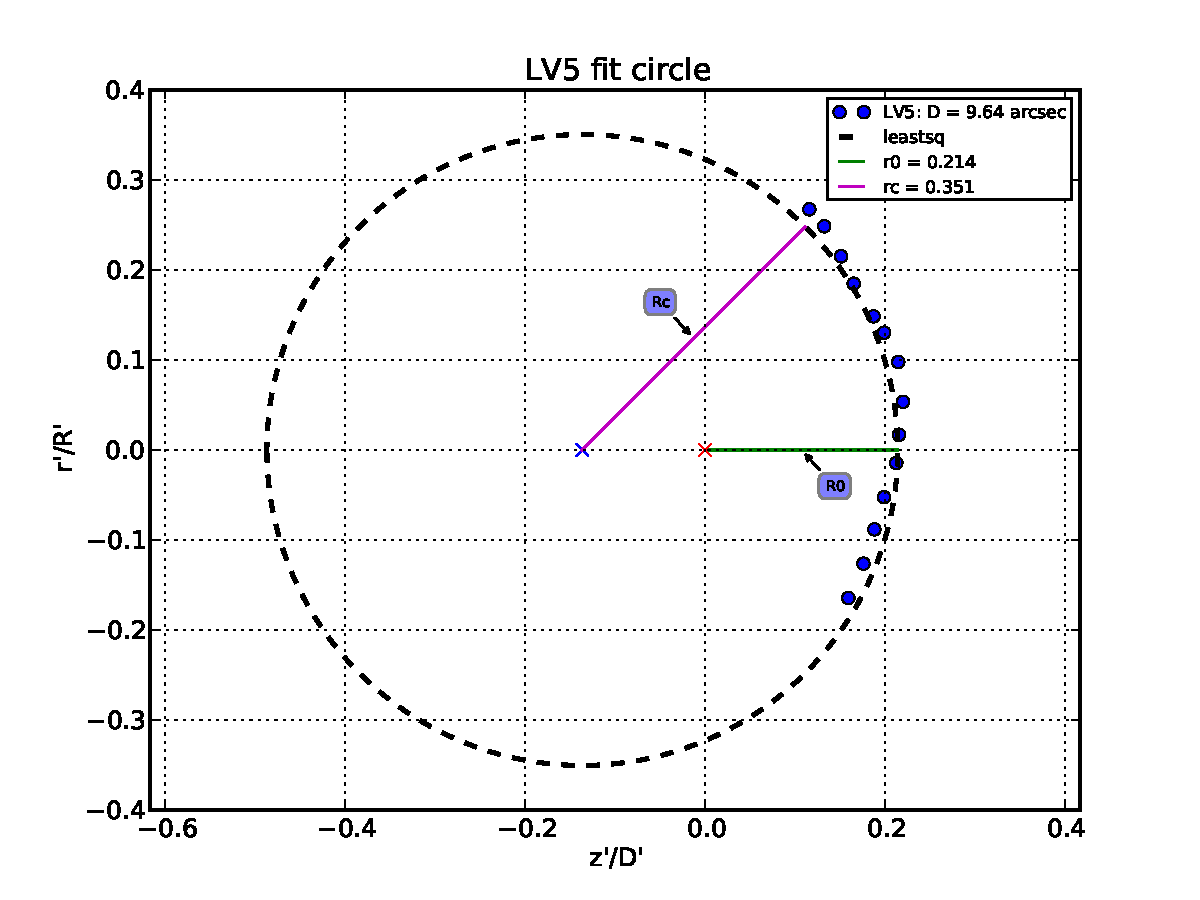
\includegraphics[width=0.5\linewidth]{LV-bowshocks-xyfancy-onaxis-OIII3a-LV5} \\
%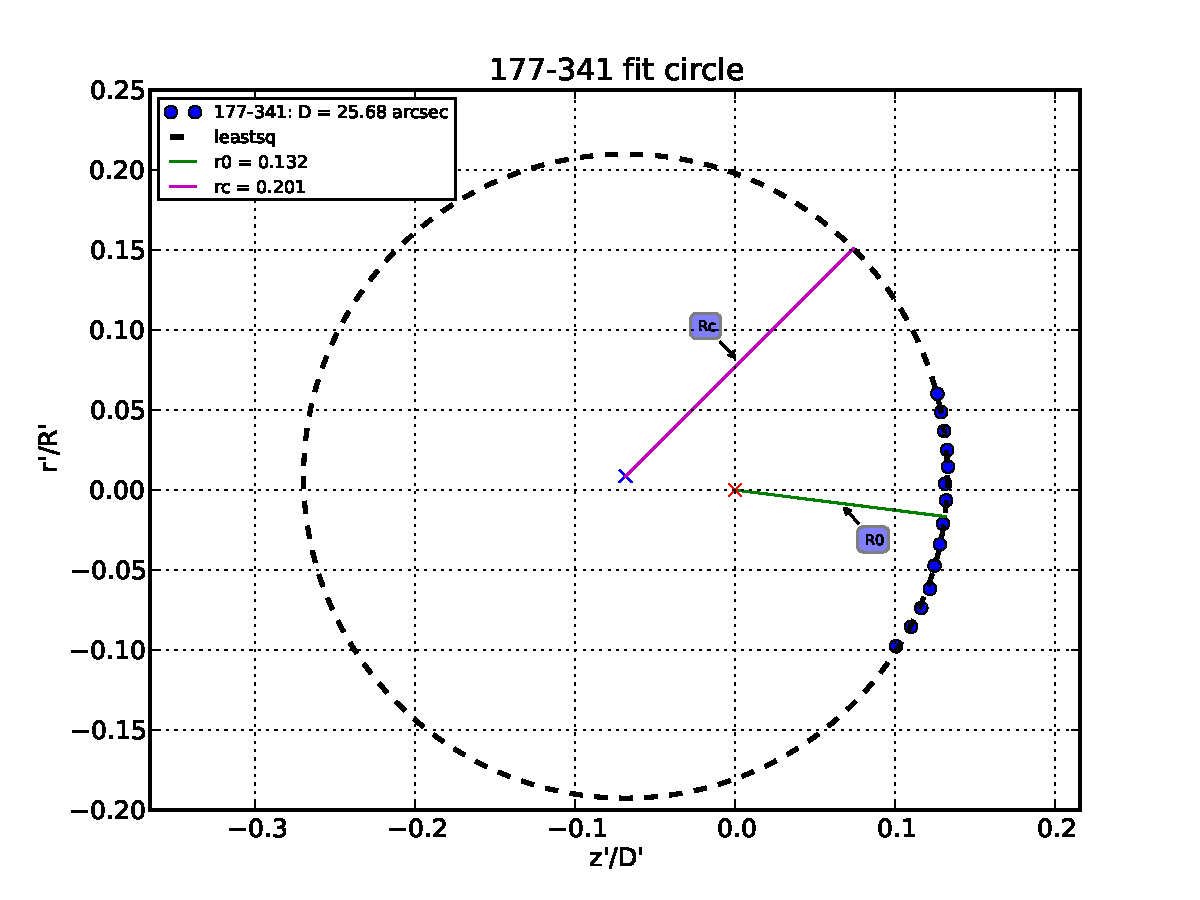
\includegraphics[width=0.5\linewidth]{LV-bowshocks-xyfancy-502epositions-177-341} & 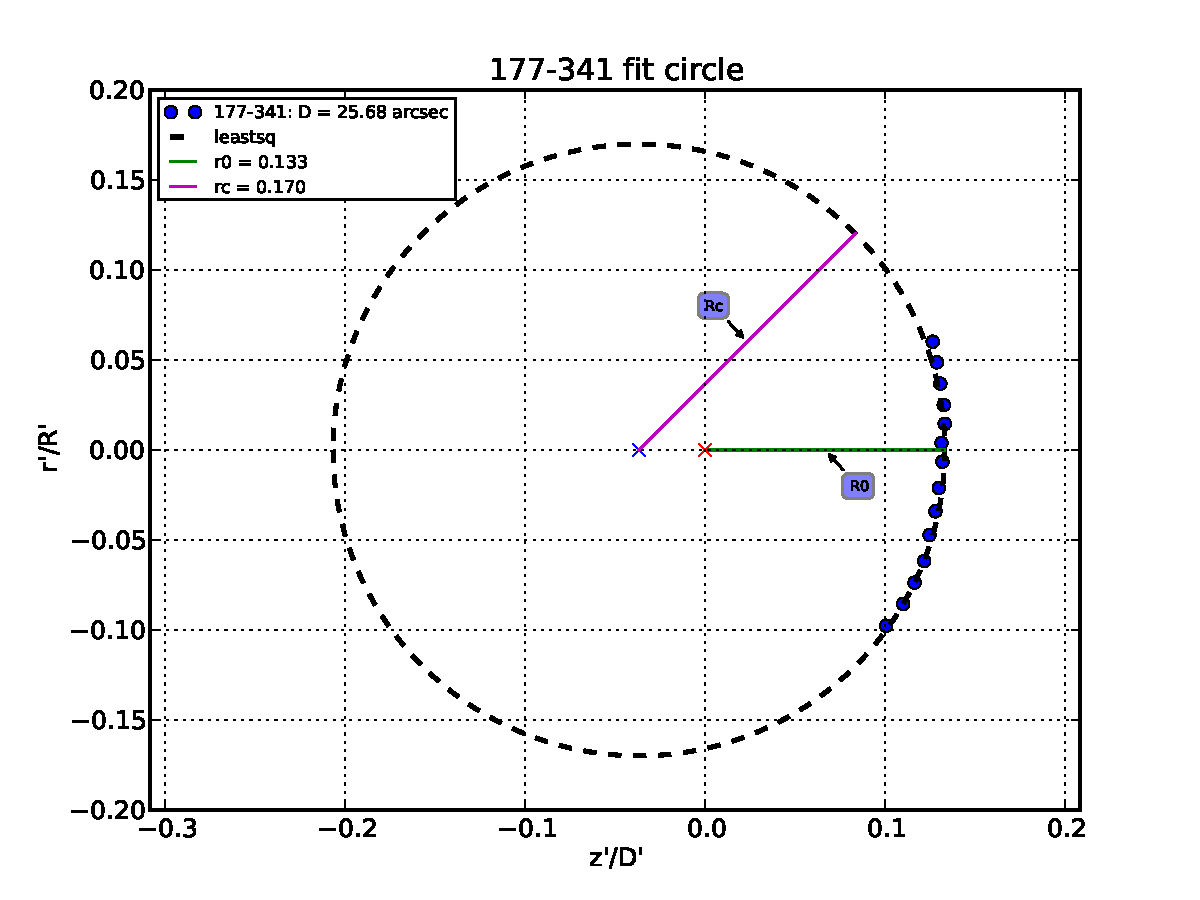
\includegraphics[width=0.5\linewidth]{LV-bowshocks-xyfancy-onaxis-502epositions-177-341}\\
%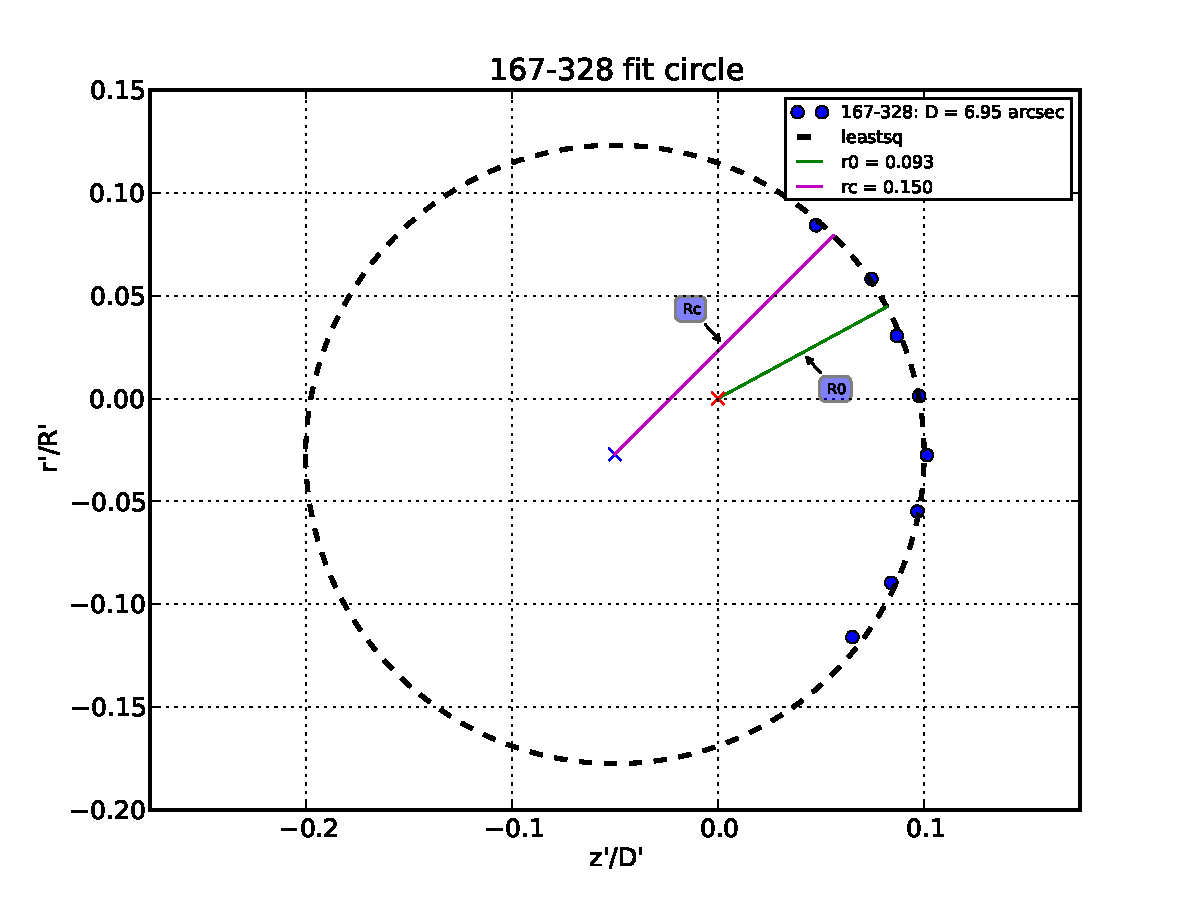
\includegraphics[width=0.5\linewidth]{LV-bowshocks-xyfancy-OIII3a-167-328} & 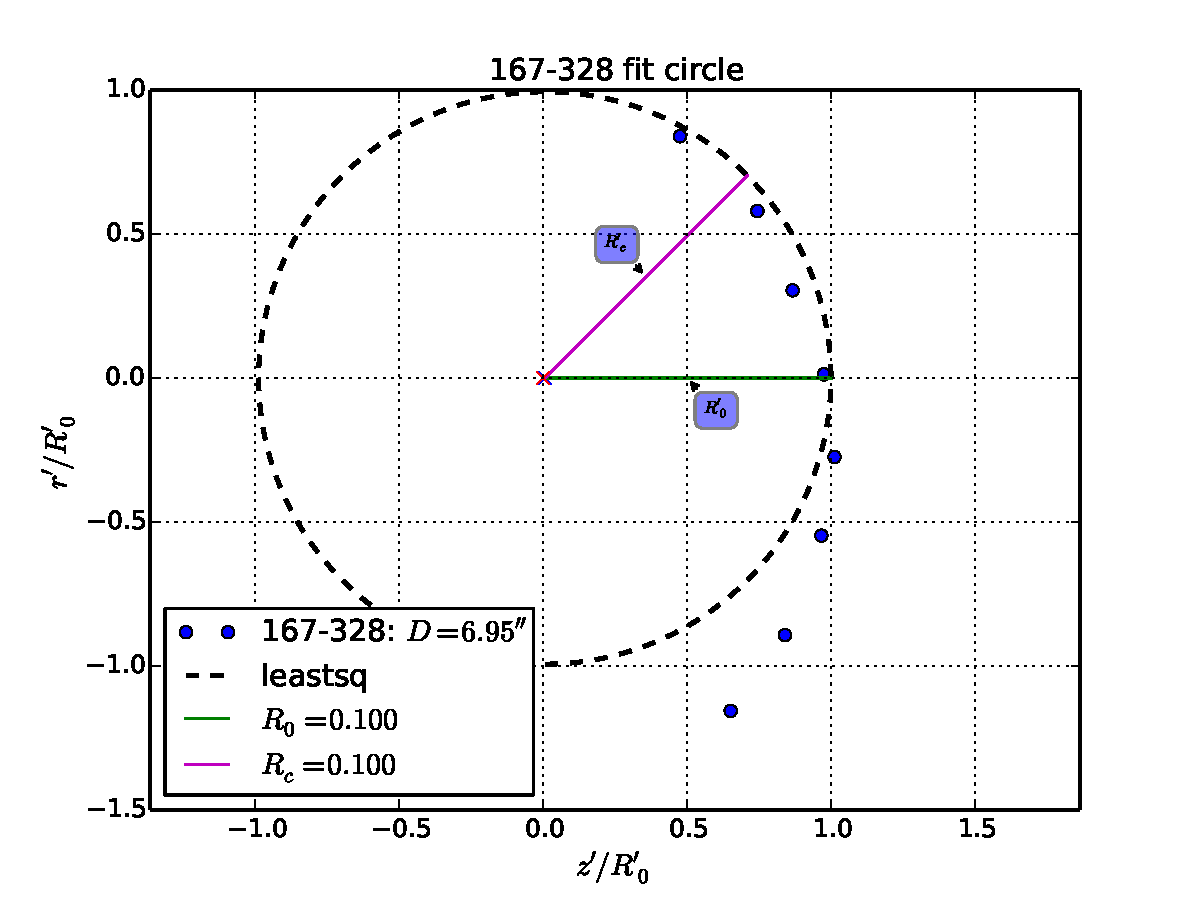
\includegraphics[width=0.5\linewidth]{LV-bowshocks-xyfancy-onaxis-OIII3a-167-328}
%\end{tabular}
%\label{fig:char-radii-obs-2}
%\caption{Continuation of figure (\ref{fig:char-radii-obs})}
%\end{figure*}
%
%\begin{figure*}
%\begin{tabular}{cc}
%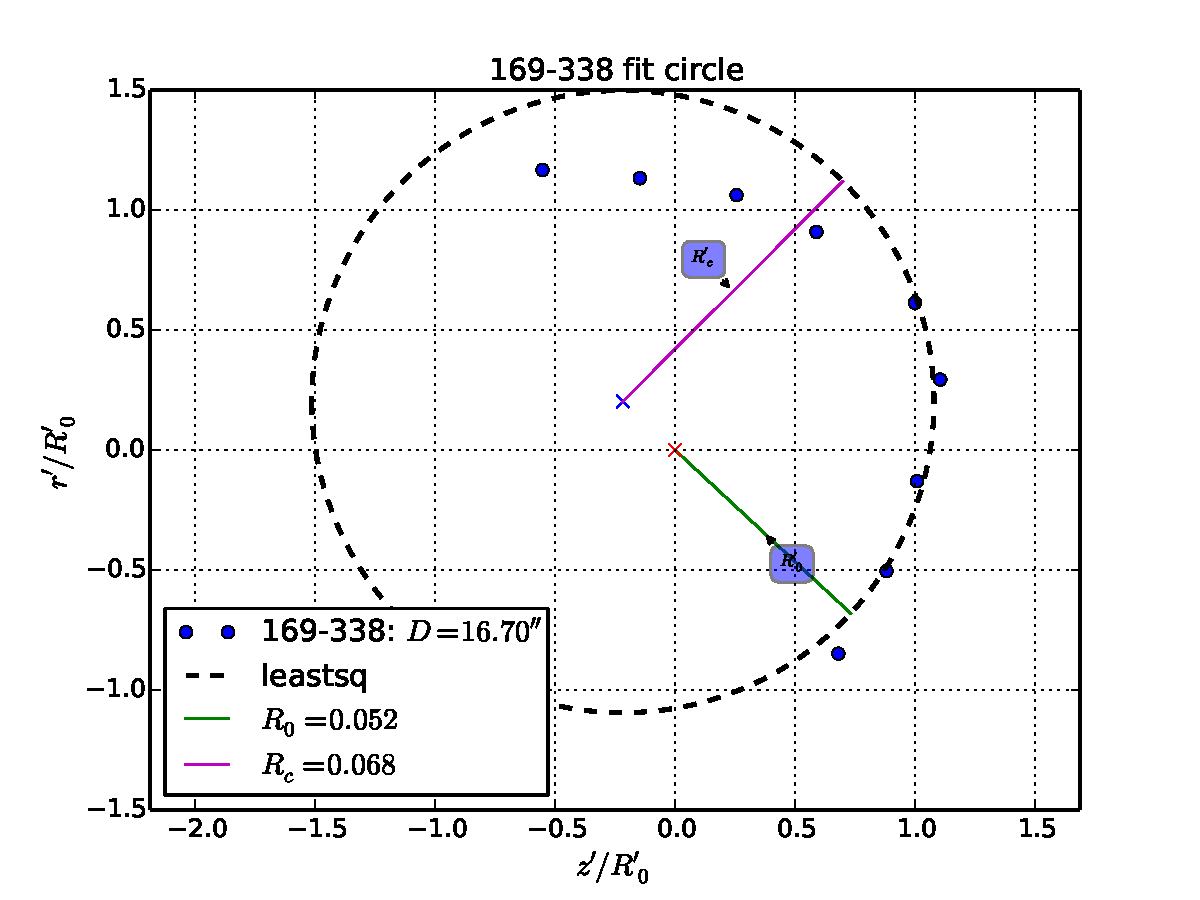
\includegraphics[width=0.5\linewidth]{LV-bowshocks-xyfancy-OIII3b-169-338} & 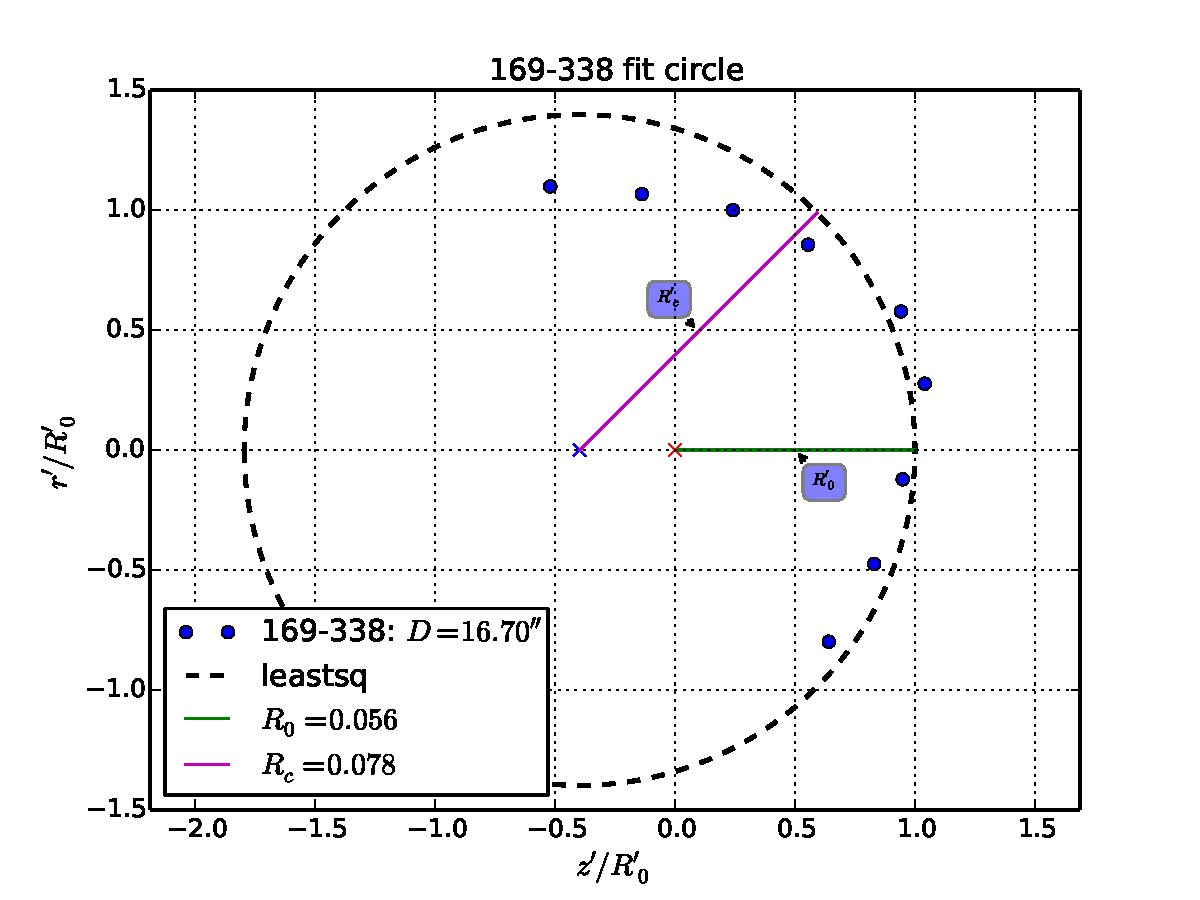
\includegraphics[width=0.5\linewidth]{LV-bowshocks-xyfancy-onaxis-OIII3b-169-338} \\
%\includegraphics[width=0.5\linewidth]{LV-bowshocks-xyfancy-OIII3b-189-329} & 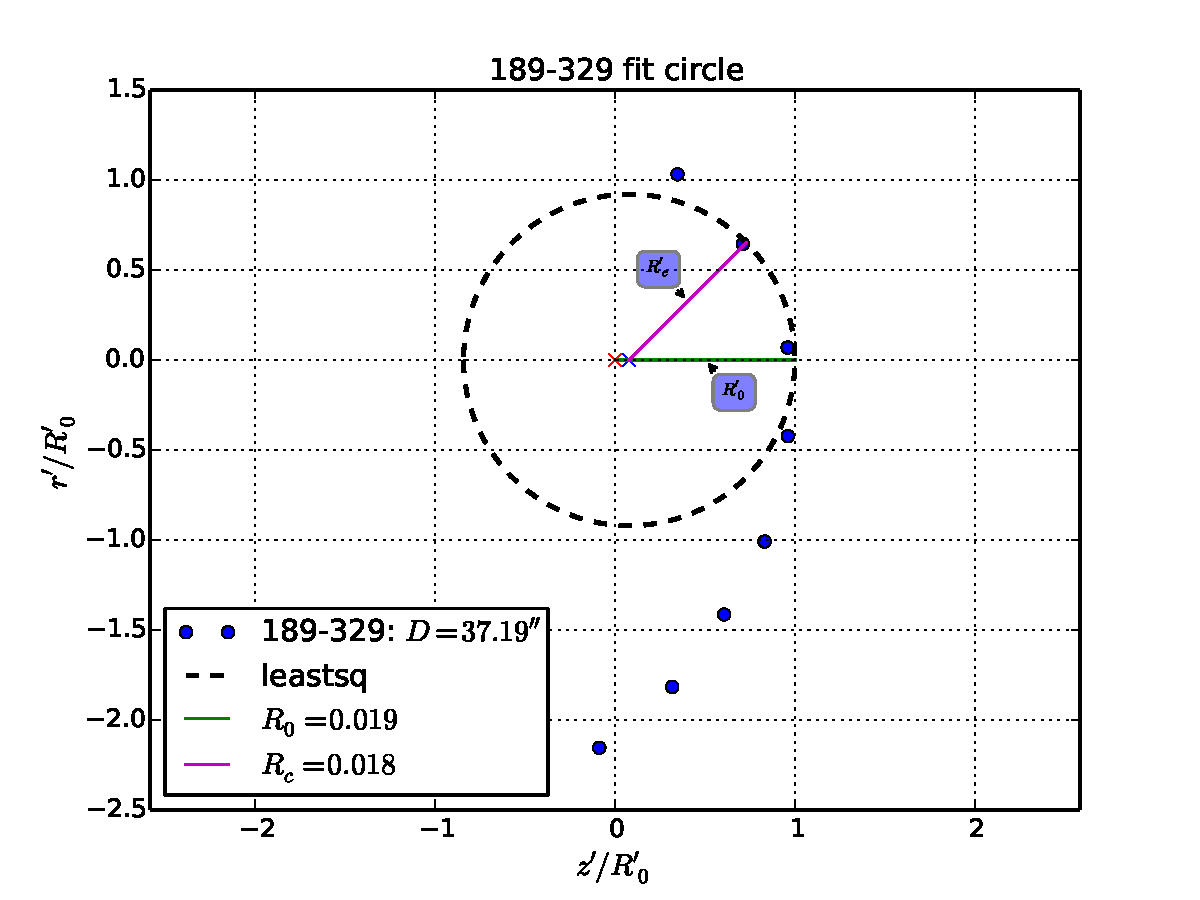
\includegraphics[width=0.5\linewidth]{LV-bowshocks-xyfancy-onaxis-OIII3b-189-329}\\
%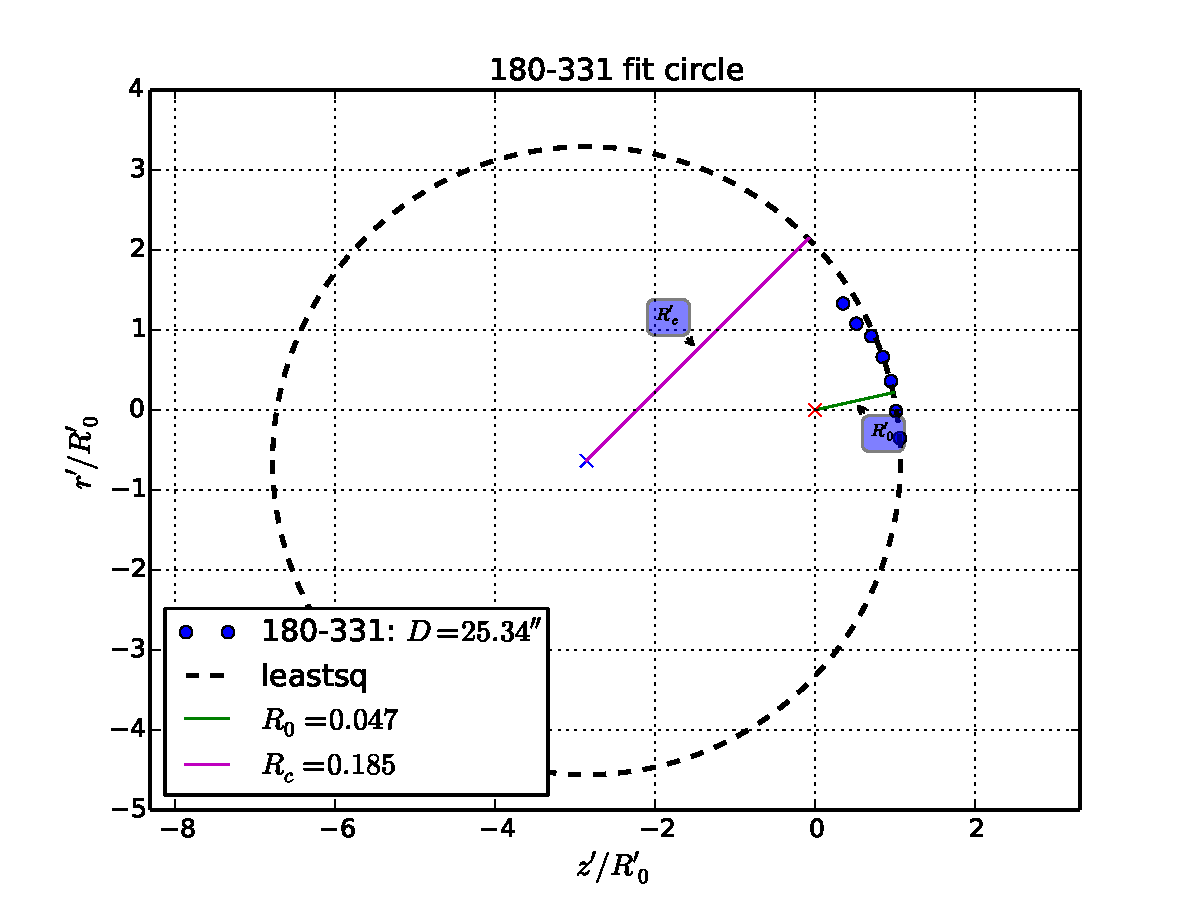
\includegraphics[width=0.5\linewidth]{LV-bowshocks-xyfancy-OIII3a-180-331} & 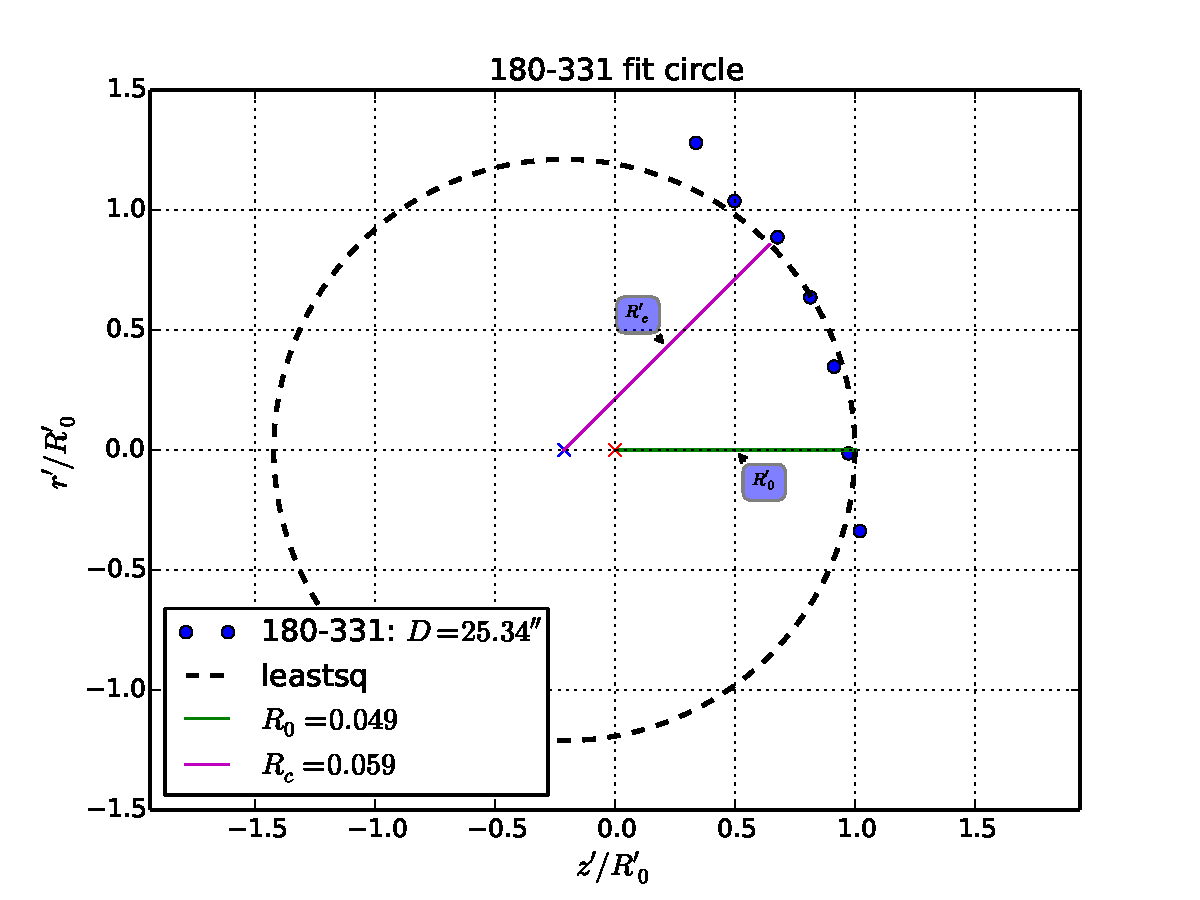
\includegraphics[width=0.5\linewidth]{LV-bowshocks-xyfancy-onaxis-OIII3a-180-331}
%\end{tabular}
%\label{fig:char-radii-obs-3}
%\caption{Continuation of figure (\ref{fig:char-radii-obs}), (new sample)}
%\end{figure*}


%%% Local Variables:
%%% mode: latex
%%% TeX-master: "proplyd-bowshocks"
%%% End:
